% Options for packages loaded elsewhere
\PassOptionsToPackage{unicode}{hyperref}
\PassOptionsToPackage{hyphens}{url}
%
\documentclass[
]{article}
\usepackage{lmodern}
\usepackage{amssymb,amsmath}
\usepackage{ifxetex,ifluatex}
\ifnum 0\ifxetex 1\fi\ifluatex 1\fi=0 % if pdftex
  \usepackage[T1]{fontenc}
  \usepackage[utf8]{inputenc}
  \usepackage{textcomp} % provide euro and other symbols
\else % if luatex or xetex
  \usepackage{unicode-math}
  \defaultfontfeatures{Scale=MatchLowercase}
  \defaultfontfeatures[\rmfamily]{Ligatures=TeX,Scale=1}
\fi
% Use upquote if available, for straight quotes in verbatim environments
\IfFileExists{upquote.sty}{\usepackage{upquote}}{}
\IfFileExists{microtype.sty}{% use microtype if available
  \usepackage[]{microtype}
  \UseMicrotypeSet[protrusion]{basicmath} % disable protrusion for tt fonts
}{}
\makeatletter
\@ifundefined{KOMAClassName}{% if non-KOMA class
  \IfFileExists{parskip.sty}{%
    \usepackage{parskip}
  }{% else
    \setlength{\parindent}{0pt}
    \setlength{\parskip}{6pt plus 2pt minus 1pt}}
}{% if KOMA class
  \KOMAoptions{parskip=half}}
\makeatother
\usepackage{xcolor}
\IfFileExists{xurl.sty}{\usepackage{xurl}}{} % add URL line breaks if available
\IfFileExists{bookmark.sty}{\usepackage{bookmark}}{\usepackage{hyperref}}
\hypersetup{
  pdftitle={The GHap Package (Version 2.0.0)},
  pdfauthor={Yuri Tani Utsunomiya, Marco Milanesi and Mario Barbato},
  hidelinks,
  pdfcreator={LaTeX via pandoc}}
\urlstyle{same} % disable monospaced font for URLs
\usepackage[margin=1in]{geometry}
\usepackage{color}
\usepackage{fancyvrb}
\newcommand{\VerbBar}{|}
\newcommand{\VERB}{\Verb[commandchars=\\\{\}]}
\DefineVerbatimEnvironment{Highlighting}{Verbatim}{commandchars=\\\{\}}
% Add ',fontsize=\small' for more characters per line
\newenvironment{Shaded}{}{}
\newcommand{\AlertTok}[1]{\textcolor[rgb]{1.00,0.00,0.00}{#1}}
\newcommand{\AnnotationTok}[1]{\textcolor[rgb]{0.00,0.50,0.00}{#1}}
\newcommand{\AttributeTok}[1]{#1}
\newcommand{\BaseNTok}[1]{#1}
\newcommand{\BuiltInTok}[1]{#1}
\newcommand{\CharTok}[1]{\textcolor[rgb]{0.00,0.50,0.50}{#1}}
\newcommand{\CommentTok}[1]{\textcolor[rgb]{0.00,0.50,0.00}{#1}}
\newcommand{\CommentVarTok}[1]{\textcolor[rgb]{0.00,0.50,0.00}{#1}}
\newcommand{\ConstantTok}[1]{#1}
\newcommand{\ControlFlowTok}[1]{\textcolor[rgb]{0.00,0.00,1.00}{#1}}
\newcommand{\DataTypeTok}[1]{#1}
\newcommand{\DecValTok}[1]{#1}
\newcommand{\DocumentationTok}[1]{\textcolor[rgb]{0.00,0.50,0.00}{#1}}
\newcommand{\ErrorTok}[1]{\textcolor[rgb]{1.00,0.00,0.00}{\textbf{#1}}}
\newcommand{\ExtensionTok}[1]{#1}
\newcommand{\FloatTok}[1]{#1}
\newcommand{\FunctionTok}[1]{#1}
\newcommand{\ImportTok}[1]{#1}
\newcommand{\InformationTok}[1]{\textcolor[rgb]{0.00,0.50,0.00}{#1}}
\newcommand{\KeywordTok}[1]{\textcolor[rgb]{0.00,0.00,1.00}{#1}}
\newcommand{\NormalTok}[1]{#1}
\newcommand{\OperatorTok}[1]{#1}
\newcommand{\OtherTok}[1]{\textcolor[rgb]{1.00,0.25,0.00}{#1}}
\newcommand{\PreprocessorTok}[1]{\textcolor[rgb]{1.00,0.25,0.00}{#1}}
\newcommand{\RegionMarkerTok}[1]{#1}
\newcommand{\SpecialCharTok}[1]{\textcolor[rgb]{0.00,0.50,0.50}{#1}}
\newcommand{\SpecialStringTok}[1]{\textcolor[rgb]{0.00,0.50,0.50}{#1}}
\newcommand{\StringTok}[1]{\textcolor[rgb]{0.00,0.50,0.50}{#1}}
\newcommand{\VariableTok}[1]{#1}
\newcommand{\VerbatimStringTok}[1]{\textcolor[rgb]{0.00,0.50,0.50}{#1}}
\newcommand{\WarningTok}[1]{\textcolor[rgb]{0.00,0.50,0.00}{\textbf{#1}}}
\usepackage{graphicx,grffile}
\makeatletter
\def\maxwidth{\ifdim\Gin@nat@width>\linewidth\linewidth\else\Gin@nat@width\fi}
\def\maxheight{\ifdim\Gin@nat@height>\textheight\textheight\else\Gin@nat@height\fi}
\makeatother
% Scale images if necessary, so that they will not overflow the page
% margins by default, and it is still possible to overwrite the defaults
% using explicit options in \includegraphics[width, height, ...]{}
\setkeys{Gin}{width=\maxwidth,height=\maxheight,keepaspectratio}
% Set default figure placement to htbp
\makeatletter
\def\fps@figure{htbp}
\makeatother
\setlength{\emergencystretch}{3em} % prevent overfull lines
\providecommand{\tightlist}{%
  \setlength{\itemsep}{0pt}\setlength{\parskip}{0pt}}
\setcounter{secnumdepth}{-\maxdimen} % remove section numbering
\usepackage{float}

\title{The \textbf{GHap} Package (Version 2.0.0)}
\author{Yuri Tani Utsunomiya, Marco Milanesi and Mario Barbato}
\date{11 Sep 2020}

\begin{document}
\maketitle

{
\setcounter{tocdepth}{2}
\tableofcontents
}
\pagebreak

\#\#Abstract

The \textbf{GHap} R package was designed to call haplotypes from phased
SNP data. Given user-defined haplotype blocks (HapBlock), the package
identifies the different haplotype alleles (HapAllele) present in the
data and scores sample haplotype allele genotypes (HapGenotype) based on
copy number (i.e., 0, 1 or 2 copies). \textbf{GHap} is an acronym for
\textbf{G}enome-wide \textbf{Hap}lotyping, and is pronounced
\textbf{G}-\textbf{Hap}, not gap (although it is intended to fill the
gap of haplotype analyses). Apart from its core functionality, the
package also supports phenotype-haplotype association analyses as well
as machine learning-based predictions of local and global ancestry.

\pagebreak

\#\#Tutorial 1 - Importing phased data

Example input files can be created using the command:

\begin{Shaded}
\begin{Highlighting}[]
\CommentTok{# Copy the example data in the current working directory}
\KeywordTok{library}\NormalTok{(GHap)}
\NormalTok{exfiles <-}\StringTok{ }\KeywordTok{ghap.makefile}\NormalTok{()}
\KeywordTok{file.copy}\NormalTok{(}\DataTypeTok{from =}\NormalTok{ exfiles, }\DataTypeTok{to =} \StringTok{"./"}\NormalTok{)}
\end{Highlighting}
\end{Shaded}

The dataset comprises genotypes from the International HapMap Project
Phase 3 (The International HapMap 3 Consortium, 2010), which includes
1,011 subjects (from 11 populations) and 20,000 SNPs (randomly sampled
from chromosome 2) mapped to the NCBI build 36 (hg18) assembly.

Since version 2.0.0, GHap adopted binary input files for both improved
performance and economic data storage. In order to compress the data
into a binary file, the user can run:

\begin{Shaded}
\begin{Highlighting}[]
\CommentTok{# Compress phase data}
\KeywordTok{ghap.compress}\NormalTok{(}\DataTypeTok{input.file =} \StringTok{"human"}\NormalTok{, }\DataTypeTok{out.file =} \StringTok{"human"}\NormalTok{)}
\end{Highlighting}
\end{Shaded}

The \texttt{ghap.loadphase()} function is responsible for loading phased
chromosomes from an input file and converting them into a native
\textbf{GHap.phase} object. A detailed describtion of this object can be
found in the documentation of the function. To load the example data in
the package we can run:

\begin{Shaded}
\begin{Highlighting}[]
\CommentTok{#Load phase object}
\NormalTok{phase <-}\StringTok{ }\KeywordTok{ghap.loadphase}\NormalTok{(}\StringTok{"human"}\NormalTok{)}
\CommentTok{#   Reading in marker map information... Done.}
\CommentTok{#   A total of 20000 markers were found in 1 chromosomes.}
\CommentTok{#   Reading in sample information... Done.}
\CommentTok{#   A total of 1011 individuals were found in 11 populations.}
\CommentTok{#   Checking integrity of phased genotypes... Done.}
\CommentTok{#   Your GHap.phase object was successfully created without apparent errors.}
\end{Highlighting}
\end{Shaded}

Although the example data contains data for a single chromosome, the
current version of the package supports multiple chromosomes.

\pagebreak

\#\#Tutorial 2 - Subsetting phased objects

The \texttt{ghap.subsetphase()} function can take any combination of
markers and individuals and subset the \textbf{GHap.phase} object. This
is achieved by setting undesired markers and individuals to
\textbf{FALSE}. Inactivated individuals and markers are then ignored by
all other functions taking a \textbf{GHap.phase} object as input.

For instance, we know that markers with low polymorphic information
content may result in rare HapAlleles. If downstream analyses do not
benefit from rare HapAlleles (e.g., haplotype association), it may be
advantageous to prune these markers out prior to haplotyping. The code
below shows how to subset markers with a minor allele frequency of at
least 5\%:

\begin{Shaded}
\begin{Highlighting}[]
\CommentTok{# Subset data - markers with maf > 0.05}
\NormalTok{maf <-}\StringTok{ }\KeywordTok{ghap.freq}\NormalTok{(phase, }\DataTypeTok{type=}\StringTok{"maf"}\NormalTok{, }\DataTypeTok{ncores =} \DecValTok{1}\NormalTok{)}
\NormalTok{markers <-}\StringTok{ }\KeywordTok{names}\NormalTok{(maf)[}\KeywordTok{which}\NormalTok{(maf }\OperatorTok{>}\StringTok{ }\FloatTok{0.05}\NormalTok{)]}
\NormalTok{phase <-}\StringTok{ }\KeywordTok{ghap.subsetphase}\NormalTok{(phase, }\KeywordTok{unique}\NormalTok{(phase}\OperatorTok{$}\NormalTok{id), markers)}
\CommentTok{#   Subsetting 1011 individuals and 17267 markers... Done.}
\CommentTok{#   Final data contains 1011 individuals and 17267 markers.}
\end{Highlighting}
\end{Shaded}

\pagebreak

\#\#Tutorial 3 - Haplotyping

In principle, the user can provide the coordinates of any arbitrary
haplotype block (HapBlock). In \textbf{GHap}, we provide means to
generate coordinates for HapBlocks based on sliding windows of markers.
This strategy is particularly useful in genome-wide scans.

\begin{Shaded}
\begin{Highlighting}[]
\CommentTok{# Generate blocks of 5 markers sliding 5 markers at a time}
\NormalTok{blocks.mkr <-}\StringTok{ }\KeywordTok{ghap.blockgen}\NormalTok{(phase, }\DataTypeTok{windowsize =} \DecValTok{5}\NormalTok{, }\DataTypeTok{slide =} \DecValTok{5}\NormalTok{, }\DataTypeTok{unit =} \StringTok{"marker"}\NormalTok{)}

\CommentTok{# Generate blocks of 100 kb sliding 100 kb at a time}
\NormalTok{blocks.kb <-}\StringTok{ }\KeywordTok{ghap.blockgen}\NormalTok{(phase, }\DataTypeTok{windowsize =} \DecValTok{100}\NormalTok{, }\DataTypeTok{slide =} \DecValTok{100}\NormalTok{, }\DataTypeTok{unit =} \StringTok{"kbp"}\NormalTok{)}
\end{Highlighting}
\end{Shaded}

By default all blocks are constrained to a minimum of two markers. This
behaviour can be adjusted by setting the \emph{nsnp} argument to a
different value. The extent of overlap between consecutive blocks can be
controlled via the \emph{slide} argument, depending on how fine the user
wishes the genome-wide scan to be. Once HapBlocks have been defined,
haplotype genotypes (HapGenotypes) can be determined:

\begin{Shaded}
\begin{Highlighting}[]
\CommentTok{# Generate matrix of haplotype genotypes}
\KeywordTok{ghap.haplotyping}\NormalTok{(phase, blocks.mkr, }\DataTypeTok{outfile =} \StringTok{"human"}\NormalTok{, }\DataTypeTok{binary =} \OtherTok{TRUE}\NormalTok{, }\DataTypeTok{ncores =} \DecValTok{1}\NormalTok{)}
\CommentTok{#   Processing 3453 blocks in:}
\CommentTok{#   1 batches of 339}
\CommentTok{#   9 batches of 346}
\CommentTok{#   3453 blocks written to file}
\end{Highlighting}
\end{Shaded}

By default all HapAlleles are included in the output. If intended, the
user can exclude the minor HapAllele by setting the \emph{drop.minor}
argument to \textbf{TRUE}. Additionally, the \emph{freq} argument allows
for exclusion of HapAlleles outside of a specified frequency range.
Control of memory usage and process parallelization is achieved through
the arguments \emph{batchsize} and \emph{ncores}.

\pagebreak

\#\#Tutorial 4 - Importing and manipulating haplotype data

After HapAlleles have been scored, the data can be loaded into R using
the \texttt{ghap.loadhaplo} function:

\begin{Shaded}
\begin{Highlighting}[]
\CommentTok{# Load haplotype genotypes}
\NormalTok{haplo <-}\StringTok{ }\KeywordTok{ghap.loadhaplo}\NormalTok{(}\StringTok{"human"}\NormalTok{)}
\CommentTok{#   Reading in haplotype allele information... Done.}
\CommentTok{#   A total of 60002 haplotype alleles were found.}
\CommentTok{#   Reading in sample information... Done.}
\CommentTok{#   A total of 1011 individuals were found in 11 populations.}
\CommentTok{#   Checking integrity of haplotype genotypes... Done.}
\CommentTok{#   Your GHap.haplo object was successfully loaded without apparent errors.}
\end{Highlighting}
\end{Shaded}

Similar to the \textbf{GHap.phase} object, the user can also subset
\textbf{GHap.haplo} objects. For instance:

\begin{Shaded}
\begin{Highlighting}[]
\CommentTok{# Randomly select 500 individuals}
\NormalTok{ids <-}\StringTok{ }\KeywordTok{sample}\NormalTok{(}\DataTypeTok{x =}\NormalTok{ haplo}\OperatorTok{$}\NormalTok{id, }\DataTypeTok{size =} \DecValTok{500}\NormalTok{, }\DataTypeTok{replace =} \OtherTok{FALSE}\NormalTok{)}

\CommentTok{# Subset data}
\NormalTok{haplo.sub <-}\StringTok{ }\KeywordTok{ghap.subsethaplo}\NormalTok{(haplo,ids,haplo}\OperatorTok{$}\NormalTok{allele.in)}
\CommentTok{#   Subsetting 500 individuals and 60002 haplotype alleles... Done.}
\CommentTok{#   Final data contains 500 individuals and 60002 haplotype alleles.}

\CommentTok{# Restore selection of the entire data}
\NormalTok{haplo.sub <-}\StringTok{ }\KeywordTok{ghap.subsethaplo}\NormalTok{(haplo,}\KeywordTok{unique}\NormalTok{(haplo}\OperatorTok{$}\NormalTok{id),}\KeywordTok{rep}\NormalTok{(}\OtherTok{TRUE}\NormalTok{,}\DataTypeTok{times=}\NormalTok{haplo}\OperatorTok{$}\NormalTok{nalleles))}
\CommentTok{#   Subsetting 1011 individuals and 60002 haplotype alleles... Done.}
\CommentTok{#   Final data contains 1011 individuals and 60002 haplotype alleles.}
\end{Highlighting}
\end{Shaded}

\pagebreak

\#\#Tutorial 5 - Haplotype statistics

For each HapAllele, the \texttt{ghap.hapstats} function retrieves
absolute and relative frequencies, expected and observed number of
homozygotes, and different tests for deficit of homozygotes in
comparison to Hardy-Weinberg Equilibrium (HWE) expectations.

\begin{Shaded}
\begin{Highlighting}[]
\NormalTok{hapstats <-}\StringTok{ }\KeywordTok{ghap.hapstats}\NormalTok{(haplo, }\DataTypeTok{ncores =} \DecValTok{1}\NormalTok{)}
\CommentTok{#   Processing 60002 HapAlleles in 10 batches.}
\CommentTok{#   Inactive alleles will be ignored.}
\CommentTok{#   60002 alleles processed}
\KeywordTok{str}\NormalTok{(hapstats)}
\CommentTok{#   'data.frame':   60002 obs. of  14 variables:}
\CommentTok{#    $ BLOCK   : chr  "CHR2_B1" "CHR2_B1" "CHR2_B1" "CHR2_B1" ...}
\CommentTok{#    $ CHR     : chr  "2" "2" "2" "2" ...}
\CommentTok{#    $ BP1     : num  18228 18228 18228 18228 18228 ...}
\CommentTok{#    $ BP2     : num  75360 75360 75360 75360 75360 ...}
\CommentTok{#    $ ALLELE  : chr  "ATAGT" "ATAAC" "ATGGC" "GGAAC" ...}
\CommentTok{#    $ N       : num  2 4 5 10 42 ...}
\CommentTok{#    $ FREQ    : num  0.000989 0.001978 0.002473 0.004946 0.020772 ...}
\CommentTok{#    $ O.HOM   : num  0 0 0 0 0 1 14 17 14 524 ...}
\CommentTok{#    $ O.HET   : num  2 4 5 10 42 56 123 142 170 328 ...}
\CommentTok{#    $ E.HOM   : num  0.000989 0.003956 0.006182 0.024728 0.436202 ...}
\CommentTok{#    $ RATIO   : num  1 1 1.01 1.02 1.44 ...}
\CommentTok{#    $ BIN.logP: num  0.00043 0.00172 0.00268 0.01074 0.18948 ...}
\CommentTok{#    $ POI.logP: num  0.00043 0.00172 0.00268 0.01074 0.18944 ...}
\CommentTok{#    $ TYPE    : chr  "MINOR" "REGULAR" "REGULAR" "REGULAR" ...}
\end{Highlighting}
\end{Shaded}

The function also assigns a \emph{TYPE} category to each HapAllele:

``ABSENT'' = the frequency of the allele is 0;

``SINGLETON'' = unique haplotype of its block with frequency 1 (i.e.,
monomorphic block);

``MINOR'' = the least frequent haplotype of its block (in the case of
ties, only the first haplotype is marked);

``MAJOR'' = the most frequent hapotype of its block (ties are also
resolved by marking the first haplotype);

``REGULAR'' = the haplotype does not fall into any of the previous
categories.

Categories ``SINGLETON'', ``MINOR'' and ``MAJOR'' only apply to blocks
where frequencies sum to 1.

The \texttt{ghap.blockstats} function summarizes HapAllele statistics
per block and retrieves the expected heterozygosity and the number of
alleles per HapBlock. For instance:

\begin{Shaded}
\begin{Highlighting}[]
\NormalTok{blockstats <-}\StringTok{ }\KeywordTok{ghap.blockstats}\NormalTok{(hapstats, }\DataTypeTok{ncores =} \DecValTok{1}\NormalTok{)}
\KeywordTok{head}\NormalTok{(blockstats,}\DataTypeTok{n=}\DecValTok{2}\NormalTok{)}
\CommentTok{#        BLOCK CHR   BP1    BP2     EXP.H N.ALLELES}
\CommentTok{#   1  CHR2_B1   2 18228  75360 0.5128683        10}
\CommentTok{#   11 CHR2_B2   2 90190 109437 0.7139595        15}
\end{Highlighting}
\end{Shaded}

Notice that calculation of expected heterozygosity will not be reliable
when HapAlleles are prunned out by frequency during haplotyping.
Therefore, the function will return NA for blocks where HapAllele
frequencies do not sum to unity. Also, when the dataset contains
multiple populations the expected heterozygosity and the number of
alleles will be very high.

\pagebreak

\#\#Tutorial 6 - Relationship matrix and PCA

The example below computes a kinship matrix from HapGenotypes and plots
the first two eigenvectors of a principal components analysis of this
matrix. Notice that absent, singleton and minor alleles should be
excluded from computations.

\begin{Shaded}
\begin{Highlighting}[]
\CommentTok{# Exclude minor alleles and singletons}
\NormalTok{haplo <-}\StringTok{ }\KeywordTok{ghap.subsethaplo}\NormalTok{(haplo,haplo}\OperatorTok{$}\NormalTok{id, hapstats}\OperatorTok{$}\NormalTok{TYPE }\OperatorTok\StringTok{ }\KeywordTok{c}\NormalTok{(}\StringTok{"REGULAR"}\NormalTok{,}\StringTok{"MAJOR"}\NormalTok{))}
\CommentTok{#   Subsetting 1011 individuals and 56572 haplotype alleles... Done.}
\CommentTok{#   Final data contains 1011 individuals and 56572 haplotype alleles.}

\CommentTok{# Compute Kinship matrix}
\NormalTok{K <-}\StringTok{ }\KeywordTok{ghap.kinship}\NormalTok{(haplo, }\DataTypeTok{ncores =} \DecValTok{1}\NormalTok{)}
\CommentTok{#   Processing 56572 HapAlleles in 10 batches.}
\CommentTok{#   Inactive alleles will be ignored.}
\CommentTok{#   Preparing 1011 x 1011 kinship matrix.}
\CommentTok{#   56572 HapAlleles processed.}

\CommentTok{# PCA analysis}
\NormalTok{pca <-}\StringTok{ }\KeywordTok{ghap.pca}\NormalTok{(haplo,K)}

\CommentTok{# Plot}
\KeywordTok{plot}\NormalTok{(}\DataTypeTok{x=}\NormalTok{pca}\OperatorTok{$}\NormalTok{eigenvec}\OperatorTok{$}\NormalTok{PC1, }\DataTypeTok{y=}\NormalTok{pca}\OperatorTok{$}\NormalTok{eigenvec}\OperatorTok{$}\NormalTok{PC2, }\DataTypeTok{xlab=}\StringTok{"PC1"}\NormalTok{, }\DataTypeTok{ylab=}\StringTok{"PC2"}\NormalTok{, }\DataTypeTok{pch=}\StringTok{""}\NormalTok{)}
\NormalTok{pop <-}\StringTok{ }\NormalTok{pca}\OperatorTok{$}\NormalTok{eigenvec}\OperatorTok{$}\NormalTok{POP}
\NormalTok{pop.col <-}\StringTok{ }\KeywordTok{as.numeric}\NormalTok{(}\KeywordTok{as.factor}\NormalTok{(pop))}
\NormalTok{pop <-}\StringTok{ }\KeywordTok{sort}\NormalTok{(}\KeywordTok{unique}\NormalTok{(pop))}
\KeywordTok{legend}\NormalTok{(}\StringTok{"bottomleft"}\NormalTok{, }\DataTypeTok{legend =}\NormalTok{ pop, }\DataTypeTok{col =} \DecValTok{1}\OperatorTok{:}\KeywordTok{length}\NormalTok{(pop), }\DataTypeTok{pch =} \DecValTok{1}\OperatorTok{:}\KeywordTok{length}\NormalTok{(pop), }\DataTypeTok{ncol =} \DecValTok{3}\NormalTok{)}
\KeywordTok{points}\NormalTok{(}\DataTypeTok{x=}\NormalTok{pca}\OperatorTok{$}\NormalTok{eigenvec}\OperatorTok{$}\NormalTok{PC1, }\DataTypeTok{y=}\NormalTok{pca}\OperatorTok{$}\NormalTok{eigenvec}\OperatorTok{$}\NormalTok{PC2, }\DataTypeTok{pch =}\NormalTok{ pop.col, }\DataTypeTok{col =}\NormalTok{ pop.col, }\DataTypeTok{cex =} \FloatTok{1.2}\NormalTok{)}
\end{Highlighting}
\end{Shaded}

\pagebreak

\#\#Tutorial 7 - Haplotype divergence analysis

The example below compares the CEU and CHB populations for HapBlocks on
chromosome 2:

\begin{Shaded}
\begin{Highlighting}[]
\CommentTok{# Compute haplotype allele statistics for each group}
\NormalTok{haplo <-}\StringTok{ }\KeywordTok{ghap.subsethaplo}\NormalTok{(haplo,haplo}\OperatorTok{$}\NormalTok{id,}\KeywordTok{rep}\NormalTok{(}\OtherTok{TRUE}\NormalTok{,}\DataTypeTok{times=}\NormalTok{haplo}\OperatorTok{$}\NormalTok{nalleles))}
\NormalTok{CHB.ids <-}\StringTok{ }\NormalTok{haplo}\OperatorTok{$}\NormalTok{id[}\KeywordTok{which}\NormalTok{(haplo}\OperatorTok{$}\NormalTok{pop}\OperatorTok{==}\StringTok{"CHB"}\NormalTok{)]}
\NormalTok{CEU.ids <-}\StringTok{ }\NormalTok{haplo}\OperatorTok{$}\NormalTok{id[}\KeywordTok{which}\NormalTok{(haplo}\OperatorTok{$}\NormalTok{pop}\OperatorTok{==}\StringTok{"CEU"}\NormalTok{)]}
\NormalTok{haplo <-}\StringTok{ }\KeywordTok{ghap.subsethaplo}\NormalTok{(haplo,CHB.ids,haplo}\OperatorTok{$}\NormalTok{allele.in)}
\NormalTok{CHB.hapstats <-}\StringTok{ }\KeywordTok{ghap.hapstats}\NormalTok{(haplo,}\DataTypeTok{ncores =} \DecValTok{1}\NormalTok{)}
\NormalTok{haplo <-}\StringTok{ }\KeywordTok{ghap.subsethaplo}\NormalTok{(haplo,CEU.ids,haplo}\OperatorTok{$}\NormalTok{allele.in)}
\NormalTok{CEU.hapstats <-}\StringTok{ }\KeywordTok{ghap.hapstats}\NormalTok{(haplo,}\DataTypeTok{ncores =} \DecValTok{1}\NormalTok{)}
\NormalTok{haplo <-}\StringTok{ }\KeywordTok{ghap.subsethaplo}\NormalTok{(haplo,}\KeywordTok{c}\NormalTok{(CHB.ids,CEU.ids),haplo}\OperatorTok{$}\NormalTok{allele.in)}
\NormalTok{TOT.hapstats <-}\StringTok{ }\KeywordTok{ghap.hapstats}\NormalTok{(haplo,}\DataTypeTok{ncores =} \DecValTok{1}\NormalTok{)}
\NormalTok{haplo <-}\StringTok{ }\KeywordTok{ghap.subsethaplo}\NormalTok{(haplo,haplo}\OperatorTok{$}\NormalTok{id,}\KeywordTok{rep}\NormalTok{(}\OtherTok{TRUE}\NormalTok{,}\DataTypeTok{times=}\NormalTok{haplo}\OperatorTok{$}\NormalTok{nalleles))}

\CommentTok{# Compute haplotype block statistics for each group}
\NormalTok{CHB.blockstats <-}\StringTok{ }\KeywordTok{ghap.blockstats}\NormalTok{(CHB.hapstats, }\DataTypeTok{ncores =} \DecValTok{1}\NormalTok{)}
\NormalTok{CEU.blockstats <-}\StringTok{ }\KeywordTok{ghap.blockstats}\NormalTok{(CEU.hapstats, }\DataTypeTok{ncores =} \DecValTok{1}\NormalTok{)}
\NormalTok{TOT.blockstats <-}\StringTok{ }\KeywordTok{ghap.blockstats}\NormalTok{(TOT.hapstats, }\DataTypeTok{ncores =} \DecValTok{1}\NormalTok{)}

\CommentTok{# Calculate Fst}
\NormalTok{fst <-}\StringTok{ }\KeywordTok{ghap.fst}\NormalTok{(CHB.blockstats, CEU.blockstats, TOT.blockstats)}

\CommentTok{# Plot results}
\NormalTok{top.fst <-}\StringTok{ }\NormalTok{fst[fst}\OperatorTok{$}\NormalTok{FST }\OperatorTok{==}\StringTok{ }\KeywordTok{max}\NormalTok{(fst}\OperatorTok{$}\NormalTok{FST, }\DataTypeTok{na.rm=}\OtherTok{TRUE}\NormalTok{),]}
\KeywordTok{plot}\NormalTok{(}
 \DataTypeTok{x =}\NormalTok{ (fst}\OperatorTok{$}\NormalTok{BP1}\OperatorTok{+}\NormalTok{fst}\OperatorTok{$}\NormalTok{BP2)}\OperatorTok{/}\FloatTok{2e+6}\NormalTok{,}
 \DataTypeTok{y =}\NormalTok{ fst}\OperatorTok{$}\NormalTok{FST, }\DataTypeTok{pch =} \StringTok{""}\NormalTok{,}
 \DataTypeTok{ylab =} \KeywordTok{expression}\NormalTok{(}\KeywordTok{paste}\NormalTok{(}\StringTok{"Haplotype "}\NormalTok{, F[ST])),}
 \DataTypeTok{xlab =} \StringTok{"Chromosome 2 (in Mb)"}\NormalTok{,}
 \DataTypeTok{ylim=}\KeywordTok{c}\NormalTok{(}\DecValTok{0}\NormalTok{,}\DecValTok{1}\NormalTok{)}
\NormalTok{)}
\KeywordTok{abline}\NormalTok{(}\DataTypeTok{v=}\FloatTok{108.7}\NormalTok{, }\DataTypeTok{col=}\StringTok{"gray"}\NormalTok{)}
\KeywordTok{points}\NormalTok{(}\DataTypeTok{x =}\NormalTok{ (fst}\OperatorTok{$}\NormalTok{BP1}\OperatorTok{+}\NormalTok{fst}\OperatorTok{$}\NormalTok{BP2)}\OperatorTok{/}\FloatTok{2e+6}\NormalTok{, }\DataTypeTok{y =}\NormalTok{ fst}\OperatorTok{$}\NormalTok{FST, }\DataTypeTok{pch =} \DecValTok{20}\NormalTok{, }\DataTypeTok{col=}\StringTok{"#471FAA99"}\NormalTok{)}
\KeywordTok{points}\NormalTok{(}\DataTypeTok{x =}\NormalTok{ (top.fst}\OperatorTok{$}\NormalTok{BP1}\OperatorTok{+}\NormalTok{top.fst}\OperatorTok{$}\NormalTok{BP2)}\OperatorTok{/}\FloatTok{2e+6}\NormalTok{, }\DataTypeTok{y =}\NormalTok{ top.fst}\OperatorTok{$}\NormalTok{FST, }\DataTypeTok{pch =} \DecValTok{20}\NormalTok{, }\DataTypeTok{col=}\StringTok{"red"}\NormalTok{)}
\KeywordTok{text}\NormalTok{(}\DataTypeTok{x =} \DecValTok{125}\NormalTok{, }\DataTypeTok{y =} \KeywordTok{max}\NormalTok{(fst}\OperatorTok{$}\NormalTok{FST, }\DataTypeTok{na.rm=}\OtherTok{TRUE}\NormalTok{), }\StringTok{"EDAR"}\NormalTok{, }\DataTypeTok{col=}\StringTok{"red"}\NormalTok{)}
\end{Highlighting}
\end{Shaded}

Ideally, similar to the case of HapAllele and HapBlock statistics, the
\(F_{ST}\) analysis should be carried out on the full set of HapAlleles,
rather than a frequency-prunned subset.

\pagebreak

\#\#Tutorial 8 - Haplotype ancestry

The package provides three methods for the prediction of haplotype
ancestry:

\textbf{GHap Unsupervised}. This method does not require a reference
sample. It is based on a combination of K-means and heuristics, and is
divided into three steps. In the first one, a random sample of seeding
markers (default value of nmarkers = 5000) is used to group all
2*nsamples haplotypes in a user-specified number of clusters (default
value of K = 2). Then, for each interrogated block, prototype alleles
(i.e., centroids) are built for every cluster using the mean of observed
haplotypes initially assigned to that cluster. Finally, each tested
haplotype is assigned to the nearest centroid (i.e., with the smallest
Euclidean distance). K-means is internally ran through the
\texttt{kmeans} function in the \textbf{stats} package.

\textbf{GHap Supervised}. This method is similar to the `unsupervised'
method, only replacing the K-means clutering step by user-defined
clusters of reference samples.

\textbf{Support Vector Machines (SVM)}. This method performs predictions
using Support Vector Machines (SVM) together with a Gaussian Radial
Basis Function (RBF) kernel. The user is required to specify a reference
sample of individuals with known ancestry labels. The reference sample
is then used to train the SVM model, which is parameterized by the C
constant of the regularization term in the Lagrange formulation (default
cost = 1) and the gamma parameter (default gamma = 1/blocksize) of the
RBF kernel. Fitting of SVM is performed internally by the \texttt{svm}
function from the \textbf{e1071} package. Test samples have the
ancestries of their HapAlleles predicted using the fitted SVM.

In all three methods, the classifiers assume exactly one ancestry per
HapBlock, such that segments encompassing breakpoints are
miss-classified as pertaining to a single ancestral origin, as opposed
to a recombinant mixture of hybrid ancestries. When any of the three
methods is ran with overlapping HapBlocks, the user should use the
\texttt{ghap.ancsmooth} function to convert HapAllele classifications
into ancestry tracks. In this case, the smoothing function interrogates
the ancestry of each overlapped segment by majority voting of all blocks
containing it. After the ancestry of all segments have been resolved,
contiguous sites sharing the same classification are converted into runs
or segments of ancestry, which comprise the final output of an ancestry
analysis. The following lines of code show an analysis of the HapMap3
data considering the three major ancestry components in human
populations: the continental blocks of Africa, Europe and Asia.

\begin{Shaded}
\begin{Highlighting}[]
\CommentTok{# Calculate marker density}
\NormalTok{mrkdist <-}\StringTok{ }\KeywordTok{diff}\NormalTok{(phase}\OperatorTok{$}\NormalTok{bp)}
\NormalTok{mrkdist <-}\StringTok{ }\NormalTok{mrkdist[}\KeywordTok{which}\NormalTok{(mrkdist }\OperatorTok{>}\StringTok{ }\DecValTok{0}\NormalTok{)]}
\NormalTok{density <-}\StringTok{ }\KeywordTok{mean}\NormalTok{(mrkdist)}

\CommentTok{# Generate blocks for admixture events up to g = 10 generations in the past}
\CommentTok{# Assuming mean block size in Morgans of 1/(2*g)}
\CommentTok{# Approximating 1 Morgan ~ 100 Mbp}
\NormalTok{g <-}\StringTok{ }\DecValTok{10}
\NormalTok{window <-}\StringTok{ }\NormalTok{(}\FloatTok{100e+6}\NormalTok{)}\OperatorTok{/}\NormalTok{(}\DecValTok{2}\OperatorTok{*}\NormalTok{g)}
\NormalTok{window <-}\StringTok{ }\KeywordTok{ceiling}\NormalTok{(window}\OperatorTok{/}\NormalTok{density)}
\NormalTok{step <-}\StringTok{ }\KeywordTok{ceiling}\NormalTok{(window}\OperatorTok{/}\DecValTok{4}\NormalTok{)}
\NormalTok{blocks <-}\StringTok{ }\KeywordTok{ghap.blockgen}\NormalTok{(phase, }\DataTypeTok{windowsize =}\NormalTok{ window, }\DataTypeTok{slide =}\NormalTok{ step, }\DataTypeTok{unit =} \StringTok{"marker"}\NormalTok{)}

\CommentTok{# Unsupervised analysis}
\NormalTok{prototypes1 <-}\StringTok{ }\KeywordTok{ghap.anctrain}\NormalTok{(}\DataTypeTok{phase =}\NormalTok{ phase, }\DataTypeTok{K =} \DecValTok{3}\NormalTok{, }\DataTypeTok{ncores =} \DecValTok{1}\NormalTok{)}
\NormalTok{hapadmix1 <-}\StringTok{ }\KeywordTok{ghap.anctest}\NormalTok{(}\DataTypeTok{phase =}\NormalTok{ phase, }\DataTypeTok{blocks =}\NormalTok{ blocks, }\DataTypeTok{prototypes =}\NormalTok{ prototypes1,}
                         \DataTypeTok{test =} \KeywordTok{unique}\NormalTok{(phase}\OperatorTok{$}\NormalTok{id), }\DataTypeTok{ncores =} \DecValTok{1}\NormalTok{)}
\NormalTok{anctracks1 <-}\StringTok{ }\KeywordTok{ghap.ancsmooth}\NormalTok{(}\DataTypeTok{phase =}\NormalTok{ phase, }\DataTypeTok{admix =}\NormalTok{ hapadmix1, }\DataTypeTok{ncores =} \DecValTok{1}\NormalTok{)}

\CommentTok{# User-defined labels}
\NormalTok{pops <-}\StringTok{ }\NormalTok{phase}\OperatorTok{$}\NormalTok{pop}
\NormalTok{labels <-}\StringTok{ }\NormalTok{pops}
\NormalTok{labels[}\KeywordTok{which}\NormalTok{(labels }\OperatorTok\StringTok{ }\KeywordTok{c}\NormalTok{(}\StringTok{"CEU"}\NormalTok{,}\StringTok{"TSI"}\NormalTok{))] <-}\StringTok{ "Europe"}
\NormalTok{labels[}\KeywordTok{which}\NormalTok{(labels }\OperatorTok\StringTok{ }\KeywordTok{c}\NormalTok{(}\StringTok{"CHB"}\NormalTok{,}\StringTok{"JPT"}\NormalTok{,}\StringTok{"CHD"}\NormalTok{))] <-}\StringTok{ "Asia"}
\NormalTok{labels[}\KeywordTok{which}\NormalTok{(labels }\OperatorTok\StringTok{ }\KeywordTok{c}\NormalTok{(}\StringTok{"YRI"}\NormalTok{,}\StringTok{"LWK"}\NormalTok{))] <-}\StringTok{ "Africa"}
\NormalTok{labels[}\KeywordTok{which}\NormalTok{(labels }\OperatorTok\StringTok{ }\KeywordTok{c}\NormalTok{(}\StringTok{"MKK"}\NormalTok{,}\StringTok{"GIH"}\NormalTok{,}\StringTok{"ASW"}\NormalTok{,}\StringTok{"MEX"}\NormalTok{))] <-}\StringTok{ "Test"}
\NormalTok{phase}\OperatorTok{$}\NormalTok{pop <-}\StringTok{ }\NormalTok{labels}
\NormalTok{train <-}\StringTok{ }\KeywordTok{unique}\NormalTok{(phase}\OperatorTok{$}\NormalTok{id[}\KeywordTok{which}\NormalTok{(phase}\OperatorTok{$}\NormalTok{pop }\OperatorTok{!=}\StringTok{ "Test"}\NormalTok{)])}
\NormalTok{test <-}\StringTok{ }\KeywordTok{unique}\NormalTok{(phase}\OperatorTok{$}\NormalTok{id)}

\CommentTok{# Supervised analysis with default parameters}
\NormalTok{prototypes2 <-}\StringTok{ }\KeywordTok{ghap.anctrain}\NormalTok{(}\DataTypeTok{phase =}\NormalTok{ phase, }\DataTypeTok{train =}\NormalTok{ train,}
                             \DataTypeTok{method =} \StringTok{"supervised"}\NormalTok{, }\DataTypeTok{ncores =} \DecValTok{1}\NormalTok{)}
\NormalTok{hapadmix2 <-}\StringTok{ }\KeywordTok{ghap.anctest}\NormalTok{(}\DataTypeTok{phase =}\NormalTok{ phase, }\DataTypeTok{blocks =}\NormalTok{ blocks, }\DataTypeTok{prototypes =}\NormalTok{ prototypes2,}
                          \DataTypeTok{test =} \KeywordTok{unique}\NormalTok{(phase}\OperatorTok{$}\NormalTok{id), }\DataTypeTok{ncores =} \DecValTok{1}\NormalTok{)}
\NormalTok{phase}\OperatorTok{$}\NormalTok{pop <-}\StringTok{ }\NormalTok{pops}
\NormalTok{anctracks2 <-}\StringTok{ }\KeywordTok{ghap.ancsmooth}\NormalTok{(}\DataTypeTok{phase =}\NormalTok{ phase, }\DataTypeTok{admix =}\NormalTok{ hapadmix2, }\DataTypeTok{ncores =} \DecValTok{1}\NormalTok{)}

\CommentTok{# SVM analysis with default parameters}
\NormalTok{phase}\OperatorTok{$}\NormalTok{pop <-}\StringTok{ }\NormalTok{labels}
\NormalTok{hapadmix3 <-}\StringTok{ }\KeywordTok{ghap.ancsvm}\NormalTok{(}\DataTypeTok{phase =}\NormalTok{ phase, }\DataTypeTok{blocks =}\NormalTok{ blocks, }\DataTypeTok{test =}\NormalTok{ test,}
                         \DataTypeTok{train =}\NormalTok{ train, }\DataTypeTok{ncores =} \DecValTok{1}\NormalTok{)}
\NormalTok{phase}\OperatorTok{$}\NormalTok{pop <-}\StringTok{ }\NormalTok{pops}
\NormalTok{anctracks3 <-}\StringTok{ }\KeywordTok{ghap.ancsmooth}\NormalTok{(}\DataTypeTok{phase =}\NormalTok{ phase, }\DataTypeTok{admix =}\NormalTok{ hapadmix3, }\DataTypeTok{ncores =} \DecValTok{1}\NormalTok{)}

\CommentTok{# List of population orders to plot}
\NormalTok{pop.order <-}\StringTok{ }\KeywordTok{vector}\NormalTok{(}\StringTok{"list"}\NormalTok{,}\DecValTok{5}\NormalTok{)}
\KeywordTok{names}\NormalTok{(pop.order) <-}\StringTok{ }\KeywordTok{c}\NormalTok{(}\StringTok{"Africa"}\NormalTok{,}\StringTok{"Europe"}\NormalTok{,}\StringTok{"East Asia"}\NormalTok{,}\StringTok{"S. Asia"}\NormalTok{,}\StringTok{"America"}\NormalTok{)}
\NormalTok{pop.order[[}\DecValTok{1}\NormalTok{]] <-}\StringTok{ }\KeywordTok{c}\NormalTok{(}\StringTok{"YRI"}\NormalTok{,}\StringTok{"LWK"}\NormalTok{,}\StringTok{"MKK"}\NormalTok{)}
\NormalTok{pop.order[[}\DecValTok{2}\NormalTok{]] <-}\StringTok{ }\KeywordTok{c}\NormalTok{(}\StringTok{"CEU"}\NormalTok{,}\StringTok{"TSI"}\NormalTok{)}
\NormalTok{pop.order[[}\DecValTok{3}\NormalTok{]] <-}\StringTok{ }\KeywordTok{c}\NormalTok{(}\StringTok{"CHB"}\NormalTok{,}\StringTok{"JPT"}\NormalTok{,}\StringTok{"CHD"}\NormalTok{)}
\NormalTok{pop.order[[}\DecValTok{4}\NormalTok{]] <-}\StringTok{ "GIH"}
\NormalTok{pop.order[[}\DecValTok{5}\NormalTok{]] <-}\StringTok{ }\KeywordTok{c}\NormalTok{(}\StringTok{"ASW"}\NormalTok{,}\StringTok{"MEX"}\NormalTok{)}

\CommentTok{# Plot results}
\KeywordTok{ghap.ancplot}\NormalTok{(}\DataTypeTok{ancsmooth =}\NormalTok{ anctracks1, }\DataTypeTok{pop.order =}\NormalTok{ pop.order, }\DataTypeTok{use.unk =} \OtherTok{FALSE}\NormalTok{)}
\KeywordTok{ghap.ancplot}\NormalTok{(}\DataTypeTok{ancsmooth =}\NormalTok{ anctracks2, }\DataTypeTok{pop.order =}\NormalTok{ pop.order, }\DataTypeTok{use.unk =} \OtherTok{FALSE}\NormalTok{)}
\KeywordTok{ghap.ancplot}\NormalTok{(}\DataTypeTok{ancsmooth =}\NormalTok{ anctracks3, }\DataTypeTok{pop.order =}\NormalTok{ pop.order, }\DataTypeTok{use.unk =} \OtherTok{FALSE}\NormalTok{)}
\end{Highlighting}
\end{Shaded}

It is also possible to summarize average ancestries per marker for a
given group of individuals using the \texttt{ghap.ancmark} function.
This is useful to screen chromosomes for loci that substantially deviate
from the average ancestry across the genome.

\begin{Shaded}
\begin{Highlighting}[]
\CommentTok{# Plot figures side by side}
\KeywordTok{par}\NormalTok{(}\DataTypeTok{mfrow=}\KeywordTok{c}\NormalTok{(}\DecValTok{3}\NormalTok{,}\DecValTok{1}\NormalTok{))}

\CommentTok{# Plot unsupervised results}
\NormalTok{ancmark1 <-}\StringTok{ }\KeywordTok{ghap.ancmark}\NormalTok{(}\DataTypeTok{phase =}\NormalTok{ phase, }\DataTypeTok{ancsmooth =}\NormalTok{ anctracks1,}
                         \DataTypeTok{ids =} \KeywordTok{unique}\NormalTok{(phase}\OperatorTok{$}\NormalTok{id[}\KeywordTok{which}\NormalTok{(phase}\OperatorTok{$}\NormalTok{pop }\OperatorTok{==}\StringTok{ "MKK"}\NormalTok{)]))}
\KeywordTok{plot}\NormalTok{(ancmark1}\OperatorTok{$}\NormalTok{BP}\OperatorTok{/}\FloatTok{1e+6}\NormalTok{, ancmark1}\OperatorTok{$}\NormalTok{K1, }\DataTypeTok{ylim =} \KeywordTok{c}\NormalTok{(}\DecValTok{0}\NormalTok{,}\DecValTok{100}\NormalTok{), }\DataTypeTok{las=}\DecValTok{1}\NormalTok{, }\DataTypeTok{type=}\StringTok{"l"}\NormalTok{, }\DataTypeTok{col=}\StringTok{"blue"}\NormalTok{,}
     \DataTypeTok{xlab =} \StringTok{"Chromosome 2 (Mbp)"}\NormalTok{, }\DataTypeTok{ylab =} \StringTok{"Ancestry (%)"}\NormalTok{, }\DataTypeTok{main =} \StringTok{"GHap unsupervised"}\NormalTok{)}
\KeywordTok{points}\NormalTok{(ancmark1}\OperatorTok{$}\NormalTok{BP}\OperatorTok{/}\FloatTok{1e+6}\NormalTok{, ancmark1}\OperatorTok{$}\NormalTok{K2, }\DataTypeTok{type=}\StringTok{"l"}\NormalTok{, }\DataTypeTok{col=}\StringTok{"red"}\NormalTok{)}
\KeywordTok{points}\NormalTok{(ancmark1}\OperatorTok{$}\NormalTok{BP}\OperatorTok{/}\FloatTok{1e+6}\NormalTok{, ancmark1}\OperatorTok{$}\NormalTok{K3, }\DataTypeTok{type=}\StringTok{"l"}\NormalTok{, }\DataTypeTok{col=}\StringTok{"green"}\NormalTok{)}
\KeywordTok{points}\NormalTok{(ancmark1}\OperatorTok{$}\NormalTok{BP}\OperatorTok{/}\FloatTok{1e+6}\NormalTok{, ancmark1}\OperatorTok{$}\NormalTok{UNK, }\DataTypeTok{type=}\StringTok{"l"}\NormalTok{, }\DataTypeTok{col=}\StringTok{"grey"}\NormalTok{)}

\CommentTok{# Plot unsupervised results}
\NormalTok{ancmark2 <-}\StringTok{ }\KeywordTok{ghap.ancmark}\NormalTok{(}\DataTypeTok{phase =}\NormalTok{ phase, }\DataTypeTok{ancsmooth =}\NormalTok{ anctracks2,}
                         \DataTypeTok{ids =} \KeywordTok{unique}\NormalTok{(phase}\OperatorTok{$}\NormalTok{id[}\KeywordTok{which}\NormalTok{(phase}\OperatorTok{$}\NormalTok{pop }\OperatorTok{==}\StringTok{ "MKK"}\NormalTok{)]))}
\KeywordTok{plot}\NormalTok{(ancmark2}\OperatorTok{$}\NormalTok{BP}\OperatorTok{/}\FloatTok{1e+6}\NormalTok{, ancmark2}\OperatorTok{$}\NormalTok{Africa, }\DataTypeTok{ylim =} \KeywordTok{c}\NormalTok{(}\DecValTok{0}\NormalTok{,}\DecValTok{100}\NormalTok{), }\DataTypeTok{las=}\DecValTok{1}\NormalTok{, }\DataTypeTok{type=}\StringTok{"l"}\NormalTok{, }\DataTypeTok{col=}\StringTok{"blue"}\NormalTok{,}
     \DataTypeTok{xlab =} \StringTok{"Chromosome 2 (Mbp)"}\NormalTok{, }\DataTypeTok{ylab =} \StringTok{"Ancestry (%)"}\NormalTok{, }\DataTypeTok{main =} \StringTok{"GHap supervised"}\NormalTok{)}
\KeywordTok{points}\NormalTok{(ancmark2}\OperatorTok{$}\NormalTok{BP}\OperatorTok{/}\FloatTok{1e+6}\NormalTok{, ancmark2}\OperatorTok{$}\NormalTok{Asia, }\DataTypeTok{type=}\StringTok{"l"}\NormalTok{, }\DataTypeTok{col=}\StringTok{"red"}\NormalTok{)}
\KeywordTok{points}\NormalTok{(ancmark2}\OperatorTok{$}\NormalTok{BP}\OperatorTok{/}\FloatTok{1e+6}\NormalTok{, ancmark2}\OperatorTok{$}\NormalTok{Europe, }\DataTypeTok{type=}\StringTok{"l"}\NormalTok{, }\DataTypeTok{col=}\StringTok{"green"}\NormalTok{)}
\KeywordTok{points}\NormalTok{(ancmark2}\OperatorTok{$}\NormalTok{BP}\OperatorTok{/}\FloatTok{1e+6}\NormalTok{, ancmark2}\OperatorTok{$}\NormalTok{UNK, }\DataTypeTok{type=}\StringTok{"l"}\NormalTok{, }\DataTypeTok{col=}\StringTok{"grey"}\NormalTok{)}

\CommentTok{# Plot SVM results}
\NormalTok{ancmark3 <-}\StringTok{ }\KeywordTok{ghap.ancmark}\NormalTok{(}\DataTypeTok{phase =}\NormalTok{ phase, }\DataTypeTok{ancsmooth =}\NormalTok{ anctracks3,}
                         \DataTypeTok{ids =} \KeywordTok{unique}\NormalTok{(phase}\OperatorTok{$}\NormalTok{id[}\KeywordTok{which}\NormalTok{(phase}\OperatorTok{$}\NormalTok{pop }\OperatorTok{==}\StringTok{ "MKK"}\NormalTok{)]))}
\KeywordTok{plot}\NormalTok{(ancmark3}\OperatorTok{$}\NormalTok{BP}\OperatorTok{/}\FloatTok{1e+6}\NormalTok{, ancmark3}\OperatorTok{$}\NormalTok{Africa, }\DataTypeTok{ylim =} \KeywordTok{c}\NormalTok{(}\DecValTok{0}\NormalTok{,}\DecValTok{100}\NormalTok{), }\DataTypeTok{las=}\DecValTok{1}\NormalTok{, }\DataTypeTok{type=}\StringTok{"l"}\NormalTok{, }\DataTypeTok{col=}\StringTok{"blue"}\NormalTok{,}
     \DataTypeTok{xlab =} \StringTok{"Chromosome 2 (Mbp)"}\NormalTok{, }\DataTypeTok{ylab =} \StringTok{"Ancestry (%)"}\NormalTok{, }\DataTypeTok{main =} \StringTok{"SVM"}\NormalTok{)}
\KeywordTok{points}\NormalTok{(ancmark3}\OperatorTok{$}\NormalTok{BP}\OperatorTok{/}\FloatTok{1e+6}\NormalTok{, ancmark3}\OperatorTok{$}\NormalTok{Asia, }\DataTypeTok{type=}\StringTok{"l"}\NormalTok{, }\DataTypeTok{col=}\StringTok{"red"}\NormalTok{)}
\KeywordTok{points}\NormalTok{(ancmark3}\OperatorTok{$}\NormalTok{BP}\OperatorTok{/}\FloatTok{1e+6}\NormalTok{, ancmark3}\OperatorTok{$}\NormalTok{Europe, }\DataTypeTok{type=}\StringTok{"l"}\NormalTok{, }\DataTypeTok{col=}\StringTok{"green"}\NormalTok{)}
\KeywordTok{points}\NormalTok{(ancmark3}\OperatorTok{$}\NormalTok{BP}\OperatorTok{/}\FloatTok{1e+6}\NormalTok{, ancmark3}\OperatorTok{$}\NormalTok{UNK, }\DataTypeTok{type=}\StringTok{"l"}\NormalTok{, }\DataTypeTok{col=}\StringTok{"grey"}\NormalTok{)}
\end{Highlighting}
\end{Shaded}

Individual ancestry tracks can be visualized with
\texttt{ghap.karyoplot} to check carrier status of segments of interest.

\begin{Shaded}
\begin{Highlighting}[]
\CommentTok{# Plot ancestry tracks}
\KeywordTok{ghap.karyoplot}\NormalTok{(}\DataTypeTok{ancsmooth =}\NormalTok{ anctracks1, }\DataTypeTok{ids =} \StringTok{"NA19835"}\NormalTok{,}
               \DataTypeTok{chr.line =} \DecValTok{11}\NormalTok{, }\DataTypeTok{plot.line =} \DecValTok{50}\NormalTok{, }\DataTypeTok{las=}\DecValTok{1}\NormalTok{)}
\KeywordTok{ghap.karyoplot}\NormalTok{(}\DataTypeTok{ancsmooth =}\NormalTok{ anctracks2, }\DataTypeTok{ids =} \StringTok{"NA19835"}\NormalTok{,}
               \DataTypeTok{chr.line =} \DecValTok{11}\NormalTok{, }\DataTypeTok{plot.line =} \DecValTok{50}\NormalTok{, }\DataTypeTok{las=}\DecValTok{1}\NormalTok{)}
\KeywordTok{ghap.karyoplot}\NormalTok{(}\DataTypeTok{ancsmooth =}\NormalTok{ anctracks3, }\DataTypeTok{ids =} \StringTok{"NA19835"}\NormalTok{,}
               \DataTypeTok{chr.line =} \DecValTok{11}\NormalTok{, }\DataTypeTok{plot.line =} \DecValTok{50}\NormalTok{, }\DataTypeTok{las=}\DecValTok{1}\NormalTok{)}
\end{Highlighting}
\end{Shaded}

Another useful feature is the possibility of exporting ancestry track
data to PLINK for admixture mapping. The \texttt{ghap.anc2plink}
function allows the user to count the number of alleles of a given
ancestry at each marker and export a genome-wide matrix in either plain
text or PLINK binary format (Purcell et al., 2007; Chang et al., 2015).
In the latter case, bed/bim/fam files are generated, where ancestry
counts 0, 1 and 2 are recoded as NN, NH and HH genotypes (N = NULL and H
= haplotype allele), as if ancestry statuses were bi-alelic markers.
This coding scheme is acceptable for any given analysis relying on
genotype counts, as long as the user specifies that the analysis should
be done using character H as the reference for counts.

\begin{Shaded}
\begin{Highlighting}[]
\CommentTok{# Output ancestry counts}
\NormalTok{phase <-}\StringTok{ }\KeywordTok{ghap.subsetphase}\NormalTok{(}\DataTypeTok{phase =}\NormalTok{ phase,}
                          \DataTypeTok{ids =} \KeywordTok{unique}\NormalTok{(phase}\OperatorTok{$}\NormalTok{id[}\KeywordTok{which}\NormalTok{(phase}\OperatorTok{$}\NormalTok{pop }\OperatorTok{==}\StringTok{ "MEX"}\NormalTok{)]),}
                          \DataTypeTok{markers =}\NormalTok{ phase}\OperatorTok{$}\NormalTok{marker)}
\KeywordTok{ghap.anc2plink}\NormalTok{(}\DataTypeTok{phase =}\NormalTok{ phase, }\DataTypeTok{ancsmooth =}\NormalTok{ anctracks2, }\DataTypeTok{ancestry =} \StringTok{"Africa"}\NormalTok{,}
               \DataTypeTok{outfile =} \StringTok{"mex_africa"}\NormalTok{, }\DataTypeTok{ncores =} \DecValTok{1}\NormalTok{, }\DataTypeTok{batchsize =} \DecValTok{1000}\NormalTok{)}
\end{Highlighting}
\end{Shaded}

\pagebreak

\#\#Tutorial 9 - Linear mixed model analysis

\textbf{GHap} implements a wrapper of the \textbf{lme4} package (Bates
et al., 2015) to fit generalized linear mixed models of the form:

\[g(\mu_{\mathbf{y}|\mathbf{u}}) = \mathbf{Xb} + \mathbf{Zu}\]

where \(g(.)\) is a link function, \(\mu_{\mathbf{y}|\mathbf{u}}\) is
the expectation of phenotypes conditional on random effects,
\(\mathbf{b}\) is a vector of unobserved fixed effects, \(\mathbf{X}\)
is a matrix relating phenotypes to \(\mathbf{b}\), \(\mathbf{u}\) is a
vector of random effects \(\sim N(\mathbf{0},\mathbf{K}\sigma_u^2)\),
and \(\mathbf{Z}\) is an incidence matrix relating phenotypes to
\(\mathbf{u}\). Random effects can be partitioned into subgroups with
different covariance matrices. For instance, if we let \(\mathbf{K}\) be
the HapAllele relationship matrix, then \(\mathbf{u}\) becomes the
HapAllele-based polygenic effects/breeding values, and \(\sigma_u^2\)
becomes the variance due to HapAlleles. Importantly, any arbitrary
\(\mathbf{K}\) matrix is admitted, such that one may fit models
combining pedigree and haplotype relationships (e.g., single-step GWAS
analysis, see Wang et al., 2012).

In the example below we simulate a quantitative trait in Europeans with
50\% heritability, where two major HapAlleles account for 50\% of the
genetic variance. Repeated records are taken for each individual.
However, the dataset is unbalanced, such that subjects can have between
0 and 30 measurements.

\begin{Shaded}
\begin{Highlighting}[]
\CommentTok{# Subset common haplotypes in Europeans}
\NormalTok{EUR.ids <-}\StringTok{ }\NormalTok{haplo}\OperatorTok{$}\NormalTok{id[}\KeywordTok{which}\NormalTok{(haplo}\OperatorTok{$}\NormalTok{pop }\OperatorTok\StringTok{ }\KeywordTok{c}\NormalTok{(}\StringTok{"TSI"}\NormalTok{,}\StringTok{"CEU"}\NormalTok{))]}
\NormalTok{haplo <-}\StringTok{ }\KeywordTok{ghap.subsethaplo}\NormalTok{(haplo,EUR.ids,haplo}\OperatorTok{$}\NormalTok{allele.in)}
\NormalTok{hapstats <-}\StringTok{ }\KeywordTok{ghap.hapstats}\NormalTok{(haplo, }\DataTypeTok{ncores =} \DecValTok{1}\NormalTok{)}
\NormalTok{common <-}\StringTok{ }\NormalTok{hapstats}\OperatorTok{$}\NormalTok{TYPE }\OperatorTok\StringTok{ }\KeywordTok{c}\NormalTok{(}\StringTok{"REGULAR"}\NormalTok{,}\StringTok{"MAJOR"}\NormalTok{) }\OperatorTok{&}
\StringTok{ }\NormalTok{hapstats}\OperatorTok{$}\NormalTok{FREQ }\OperatorTok{>}\StringTok{ }\FloatTok{0.05} \OperatorTok{&}
\StringTok{ }\NormalTok{hapstats}\OperatorTok{$}\NormalTok{FREQ }\OperatorTok{<}\StringTok{ }\FloatTok{0.95}
\NormalTok{haplo <-}\StringTok{ }\KeywordTok{ghap.subsethaplo}\NormalTok{(haplo,EUR.ids,common)}

\CommentTok{#Compute relationship matrix}
\NormalTok{K <-}\StringTok{ }\KeywordTok{ghap.kinship}\NormalTok{(haplo, }\DataTypeTok{ncores =} \DecValTok{1}\NormalTok{)}

\CommentTok{# Quantitative trait with 50% heritability}
\CommentTok{# Unbalanced repeated measurements (0 to 30)}
\CommentTok{# Two major haplotypes accounting for 50% of the genetic variance}
\NormalTok{myseed <-}\StringTok{ }\DecValTok{123456789}
\KeywordTok{set.seed}\NormalTok{(myseed)}
\NormalTok{major <-}\StringTok{ }\KeywordTok{sample}\NormalTok{(}\KeywordTok{which}\NormalTok{(haplo}\OperatorTok{$}\NormalTok{allele.in }\OperatorTok{==}\StringTok{ }\OtherTok{TRUE}\NormalTok{), }\DataTypeTok{size =} \DecValTok{2}\NormalTok{)}
\NormalTok{g2 <-}\StringTok{ }\KeywordTok{runif}\NormalTok{(}\DataTypeTok{n =} \DecValTok{2}\NormalTok{, }\DataTypeTok{min =} \DecValTok{0}\NormalTok{, }\DataTypeTok{max =} \DecValTok{1}\NormalTok{)}
\NormalTok{g2 <-}\StringTok{ }\NormalTok{(g2}\OperatorTok{/}\KeywordTok{sum}\NormalTok{(g2))}\OperatorTok{*}\FloatTok{0.5}
\NormalTok{sim <-}\StringTok{ }\KeywordTok{ghap.simpheno}\NormalTok{(haplo, }\DataTypeTok{kinship =}\NormalTok{ K, }\DataTypeTok{h2 =} \FloatTok{0.5}\NormalTok{, }\DataTypeTok{g2 =}\NormalTok{ g2, }\DataTypeTok{nrep =} \DecValTok{30}\NormalTok{,}
                     \DataTypeTok{balanced =} \OtherTok{FALSE}\NormalTok{, }\DataTypeTok{major =}\NormalTok{ major, }\DataTypeTok{seed =}\NormalTok{ myseed)}

\CommentTok{#Fit model using REML}
\NormalTok{model <-}\StringTok{ }\KeywordTok{ghap.lmm}\NormalTok{(}\DataTypeTok{fixed =}\NormalTok{ phenotype }\OperatorTok{~}\StringTok{ }\DecValTok{1}\NormalTok{, }\DataTypeTok{random =} \OperatorTok{~}\StringTok{ }\NormalTok{individual,}
                  \DataTypeTok{covmat =} \KeywordTok{list}\NormalTok{(}\DataTypeTok{individual =}\NormalTok{ K), }\DataTypeTok{data =}\NormalTok{ sim}\OperatorTok{$}\NormalTok{data)}

\CommentTok{#Estimated heritability and repeatability}
\NormalTok{model}\OperatorTok{$}\NormalTok{vcp}\OperatorTok{/}\KeywordTok{sum}\NormalTok{(model}\OperatorTok{$}\NormalTok{vcp)}

\CommentTok{#True versus estimated breeding values}
\KeywordTok{plot}\NormalTok{(model}\OperatorTok{$}\NormalTok{random}\OperatorTok{$}\NormalTok{individual,sim}\OperatorTok{$}\NormalTok{u,}\DataTypeTok{xlab=}\StringTok{"Estimated BV"}\NormalTok{,}\DataTypeTok{ylab=}\StringTok{"True BV"}\NormalTok{); }\KeywordTok{abline}\NormalTok{(}\DecValTok{0}\NormalTok{,}\DecValTok{1}\NormalTok{)}
\KeywordTok{summary}\NormalTok{(}\KeywordTok{lm}\NormalTok{(sim}\OperatorTok{$}\NormalTok{u }\OperatorTok{~}\StringTok{ }\KeywordTok{as.numeric}\NormalTok{(model}\OperatorTok{$}\NormalTok{random}\OperatorTok{$}\NormalTok{individual)))}
\end{Highlighting}
\end{Shaded}

\pagebreak

\#\#Tutorial 10 - Association analysis

The \texttt{ghap.assoc()} function regresses a response variable on one
HapAllele at a time, treating HapAlleles as fixed effects. The example
below takes the simulated data from the previous tutorial and regresses
residuals and genomic estimated breeding values onto HapAlleles.

\begin{Shaded}
\begin{Highlighting}[]
\CommentTok{#HapAllele GWAS using GEBVs as response}
\NormalTok{pheno <-}\StringTok{ }\NormalTok{model}\OperatorTok{$}\NormalTok{random}\OperatorTok{$}\NormalTok{individual}
\NormalTok{gwas1 <-}\StringTok{ }\KeywordTok{ghap.assoc}\NormalTok{(}\DataTypeTok{response =}\NormalTok{ pheno, }\DataTypeTok{haplo =}\NormalTok{ haplo, }\DataTypeTok{ncores =} \DecValTok{1}\NormalTok{)}

\CommentTok{#HapAllele GWAS using GEBVs as response}
\CommentTok{#Weight observations by number of repeated measurements}
\NormalTok{pheno <-}\StringTok{ }\NormalTok{model}\OperatorTok{$}\NormalTok{random}\OperatorTok{$}\NormalTok{individual}
\NormalTok{w <-}\StringTok{ }\KeywordTok{table}\NormalTok{(sim}\OperatorTok{$}\NormalTok{data}\OperatorTok{$}\NormalTok{individual)}
\NormalTok{w <-}\StringTok{ }\NormalTok{w }\OperatorTok{+}\StringTok{ }\KeywordTok{mean}\NormalTok{(w)}
\NormalTok{w <-}\StringTok{ }\NormalTok{w[}\KeywordTok{names}\NormalTok{(pheno)]}
\NormalTok{gwas2 <-}\StringTok{ }\KeywordTok{ghap.assoc}\NormalTok{(}\DataTypeTok{response =}\NormalTok{ pheno, }\DataTypeTok{haplo =}\NormalTok{ haplo, }\DataTypeTok{ncores =} \DecValTok{1}\NormalTok{, }\DataTypeTok{weights =}\NormalTok{ w)}

\CommentTok{#HapAllele GWAS using residuals as response}
\NormalTok{pheno <-}\StringTok{ }\NormalTok{model}\OperatorTok{$}\NormalTok{residuals}
\KeywordTok{names}\NormalTok{(pheno) <-}\StringTok{ }\NormalTok{sim}\OperatorTok{$}\NormalTok{data}\OperatorTok{$}\NormalTok{individual}
\NormalTok{gwas3 <-}\StringTok{ }\KeywordTok{ghap.assoc}\NormalTok{(}\DataTypeTok{response =}\NormalTok{ pheno, }\DataTypeTok{haplo =}\NormalTok{ haplo, }\DataTypeTok{ncores =} \DecValTok{1}\NormalTok{)}

\CommentTok{#Plot results}
\KeywordTok{plot}\NormalTok{(gwas1}\OperatorTok{$}\NormalTok{BP1}\OperatorTok{/}\FloatTok{1e+6}\NormalTok{,gwas1}\OperatorTok{$}\NormalTok{logP,}\DataTypeTok{pch=}\DecValTok{20}\NormalTok{,}\DataTypeTok{col=}\StringTok{"darkgreen"}\NormalTok{,}\DataTypeTok{ylim=}\KeywordTok{c}\NormalTok{(}\DecValTok{0}\NormalTok{,}\DecValTok{20}\NormalTok{),}
     \DataTypeTok{xlab=}\StringTok{"Position (in Mb)"}\NormalTok{,}\DataTypeTok{ylab=}\KeywordTok{expression}\NormalTok{(}\OperatorTok{-}\NormalTok{log[}\DecValTok{10}\NormalTok{](p)))}
\KeywordTok{points}\NormalTok{(gwas2}\OperatorTok{$}\NormalTok{BP1}\OperatorTok{/}\FloatTok{1e+6}\NormalTok{,gwas2}\OperatorTok{$}\NormalTok{logP,}\DataTypeTok{pch=}\DecValTok{20}\NormalTok{,}\DataTypeTok{col=}\StringTok{"gray"}\NormalTok{)}
\KeywordTok{points}\NormalTok{(gwas3}\OperatorTok{$}\NormalTok{BP1}\OperatorTok{/}\FloatTok{1e+6}\NormalTok{,gwas3}\OperatorTok{$}\NormalTok{logP,}\DataTypeTok{pch=}\DecValTok{20}\NormalTok{,}\DataTypeTok{col=}\StringTok{"blue"}\NormalTok{)}
\KeywordTok{abline}\NormalTok{(}\DataTypeTok{v=}\NormalTok{haplo}\OperatorTok{$}\NormalTok{bp1[major]}\OperatorTok{/}\FloatTok{1e+6}\NormalTok{,}\DataTypeTok{lty=}\DecValTok{3}\NormalTok{)}
\KeywordTok{abline}\NormalTok{(}\DataTypeTok{h=}\OperatorTok{-}\KeywordTok{log10}\NormalTok{(}\FloatTok{0.05}\OperatorTok{/}\KeywordTok{nrow}\NormalTok{(gwas1)),}\DataTypeTok{lty=}\DecValTok{3}\NormalTok{)}
\KeywordTok{legend}\NormalTok{(}\StringTok{"topleft"}\NormalTok{,}\DataTypeTok{legend =} \KeywordTok{c}\NormalTok{(}\StringTok{"GEBVs"}\NormalTok{,}\StringTok{"weighted GEBVs"}\NormalTok{,}\StringTok{"residuals"}\NormalTok{),}
       \DataTypeTok{pch =} \DecValTok{20}\NormalTok{,}\DataTypeTok{col=}\KeywordTok{c}\NormalTok{(}\StringTok{"darkgreen"}\NormalTok{,}\StringTok{"gray"}\NormalTok{,}\StringTok{"blue"}\NormalTok{))}
\end{Highlighting}
\end{Shaded}

\pagebreak

\#\#Tutorial 11 - BLUP of haplotypes

HapAlleles can also be treated as random effects with the
\texttt{ghap.blup()} function. Random effects can be iteratively updated
through the \emph{haploweights} argument following the single-step GWAS
approach (Wang et al., 2012):

\begin{Shaded}
\begin{Highlighting}[]
\CommentTok{#BLUP GWAS}
\NormalTok{gebvs <-}\StringTok{ }\NormalTok{model}\OperatorTok{$}\NormalTok{random}\OperatorTok{$}\NormalTok{individual}
\NormalTok{gebvsw <-}\StringTok{ }\KeywordTok{table}\NormalTok{(sim}\OperatorTok{$}\NormalTok{data}\OperatorTok{$}\NormalTok{individual)}
\NormalTok{gebvsw <-}\StringTok{ }\NormalTok{gebvsw }\OperatorTok{+}\StringTok{ }\KeywordTok{mean}\NormalTok{(gebvsw)}
\NormalTok{gebvsw <-}\StringTok{ }\NormalTok{gebvsw[}\KeywordTok{names}\NormalTok{(gebvs)]}
\NormalTok{Kinv <-}\StringTok{ }\KeywordTok{ghap.kinv}\NormalTok{(K)}
\NormalTok{gwas.blup <-}\StringTok{ }\KeywordTok{ghap.blup}\NormalTok{(}\DataTypeTok{gebvs =}\NormalTok{ gebvs, }\DataTypeTok{haplo =}\NormalTok{ haplo, }\DataTypeTok{gebvsweights =}\NormalTok{ gebvsw,}
                       \DataTypeTok{ncores =} \DecValTok{1}\NormalTok{, }\DataTypeTok{invcov =}\NormalTok{ Kinv)}
\KeywordTok{plot}\NormalTok{(gwas.blup}\OperatorTok{$}\NormalTok{BP1}\OperatorTok{/}\FloatTok{1e+6}\NormalTok{,gwas.blup}\OperatorTok{$}\NormalTok{pVAR}\OperatorTok{*}\DecValTok{100}\NormalTok{,}\DataTypeTok{pch=}\DecValTok{20}\NormalTok{,}
     \DataTypeTok{xlab=}\StringTok{"Position (in Mb)"}\NormalTok{,}\DataTypeTok{ylab=}\StringTok{"Variance explained (%)"}\NormalTok{)}
\KeywordTok{abline}\NormalTok{(}\DataTypeTok{v=}\NormalTok{haplo}\OperatorTok{$}\NormalTok{bp1[major]}\OperatorTok{/}\FloatTok{1e+6}\NormalTok{)}

\CommentTok{#BLUP with one update}
\NormalTok{w <-}\StringTok{ }\NormalTok{gwas.blup}\OperatorTok{$}\NormalTok{VAR}\OperatorTok{*}\KeywordTok{nrow}\NormalTok{(gwas.blup)}
\NormalTok{K2 <-}\StringTok{ }\KeywordTok{ghap.kinship}\NormalTok{(}\DataTypeTok{haplo=}\NormalTok{haplo,}\DataTypeTok{weights =}\NormalTok{ w)}
\NormalTok{Kinv2 <-}\StringTok{ }\KeywordTok{ghap.kinv}\NormalTok{(K2)}
\NormalTok{gwas.blup2 <-}\StringTok{ }\KeywordTok{ghap.blup}\NormalTok{(}\DataTypeTok{gebvs =}\NormalTok{ gebvs, }\DataTypeTok{haplo =}\NormalTok{ haplo, }\DataTypeTok{invcov =}\NormalTok{ Kinv2, }\DataTypeTok{ncores =} \DecValTok{1}\NormalTok{,}
                       \DataTypeTok{gebvsweights =}\NormalTok{ gebvsw, }\DataTypeTok{haploweights =}\NormalTok{ w)}
\KeywordTok{plot}\NormalTok{(gwas.blup2}\OperatorTok{$}\NormalTok{BP1}\OperatorTok{/}\FloatTok{1e+6}\NormalTok{,gwas.blup2}\OperatorTok{$}\NormalTok{pVAR}\OperatorTok{*}\DecValTok{100}\NormalTok{,}\DataTypeTok{pch=}\DecValTok{20}\NormalTok{,}
     \DataTypeTok{xlab=}\StringTok{"Position (in Mb)"}\NormalTok{,}\DataTypeTok{ylab=}\StringTok{"Variance explained (%)"}\NormalTok{)}
\KeywordTok{abline}\NormalTok{(}\DataTypeTok{v=}\NormalTok{haplo}\OperatorTok{$}\NormalTok{bp1[major]}\OperatorTok{/}\FloatTok{1e+6}\NormalTok{)}
\end{Highlighting}
\end{Shaded}

\pagebreak

\#\#Tutorial 12 - Haplotype profiling

The profile for each individual is calculated as:

\[\sum_{i=1}^{m}(h_ia_i)\]

where relative to HapAllele \(i\), \(h_i\) is the number of copies and
\(a_i\) is a user-defined score. By default, if scores are provided for
only a subset of the HapAlleles, the missing alleles scores will be set
to zero. This function has the same spirit as the profiling routine
implemented in the score option in PLINK (Purcell et al., 2007; Chang et
al., 2015). This function can be useful for analyses involving
cross-validation of genomic predictions based on BLUP solutions of
HapAllele effects. Below is an example using simulated scores from a
normal distribution:

\begin{Shaded}
\begin{Highlighting}[]
\CommentTok{# Create a score data.frame}
\NormalTok{score <-}\StringTok{ }\OtherTok{NULL}
\NormalTok{score}\OperatorTok{$}\NormalTok{BLOCK <-}\StringTok{ }\NormalTok{haplo}\OperatorTok{$}\NormalTok{block}
\NormalTok{score}\OperatorTok{$}\NormalTok{CHR <-}\StringTok{ }\NormalTok{haplo}\OperatorTok{$}\NormalTok{chr}
\NormalTok{score}\OperatorTok{$}\NormalTok{BP1 <-}\StringTok{ }\NormalTok{haplo}\OperatorTok{$}\NormalTok{bp1}
\NormalTok{score}\OperatorTok{$}\NormalTok{BP2 <-}\StringTok{ }\NormalTok{haplo}\OperatorTok{$}\NormalTok{bp2}
\NormalTok{score}\OperatorTok{$}\NormalTok{ALLELE <-}\StringTok{ }\NormalTok{haplo}\OperatorTok{$}\NormalTok{allele}
\KeywordTok{set.seed}\NormalTok{(}\DecValTok{1988}\NormalTok{)}
\NormalTok{score}\OperatorTok{$}\NormalTok{SCORE <-}\StringTok{ }\KeywordTok{rnorm}\NormalTok{(}\KeywordTok{length}\NormalTok{(score}\OperatorTok{$}\NormalTok{ALLELE))}
\NormalTok{score <-}\StringTok{ }\KeywordTok{data.frame}\NormalTok{(score,}\DataTypeTok{stringsAsFactors =} \OtherTok{FALSE}\NormalTok{)}
\NormalTok{score}\OperatorTok{$}\NormalTok{CENTER <-}\StringTok{ }\DecValTok{0}
\NormalTok{score}\OperatorTok{$}\NormalTok{SCALE <-}\StringTok{ }\DecValTok{1}

\CommentTok{# Compute profiles}
\NormalTok{profile <-}\StringTok{ }\KeywordTok{ghap.profile}\NormalTok{(score, haplo, }\DataTypeTok{ncores =} \DecValTok{1}\NormalTok{)}
\KeywordTok{head}\NormalTok{(profile)}
\CommentTok{#     POP      ID    PROFILE}
\CommentTok{#   1 ASW NA19904 -38.410381}
\CommentTok{#   2 ASW NA20340 -12.250027}
\CommentTok{#   3 ASW NA20297 -45.473774}
\CommentTok{#   4 ASW NA20281  -7.360974}
\CommentTok{#   5 ASW NA20348 -36.271198}
\CommentTok{#   6 ASW NA20300  40.912226}
\end{Highlighting}
\end{Shaded}

\pagebreak

\#\#Methods 1 - Format

The supported format is composed of three files with suffix:

\textbf{.samples} = space-delimited file without header containing two
columns: Population and ID. Please notice that the Population column
serves solely for the purpose of grouping samples, so the user can
define any arbitrary family/cluster/subgroup and use as a ``population''
tag.

\textbf{.markers} = space-delimited file without header containing five
columns: Chromosome, Marker, Position (in bp), Reference Allele (A0) and
Alternative Allele (A1). Markers should be on a single chromosome and
sorted by position.

\textbf{.phase} = space-delimited file without header containing the
phased genotype matrix. The dimension of the matrix is expected to be
\(m\) x \(2n\), where \(m\) is the number of markers and \(n\) is the
number of individuals. Alleles must be coded as 0 and 1. No missing
values are allowed.

See below an example of five individuals from the ASW population with
phased genotypes for five markers on chromosome 2:

\begin{Shaded}
\begin{Highlighting}[]
\NormalTok{======================================================================}
\NormalTok{|  .samples file  |      .markers file       |      .phase file      |}
\NormalTok{======================================================================}
\NormalTok{|  ASW NA19904    |  }\DecValTok{2}\NormalTok{ rs13383216 }\DecValTok{18228}\NormalTok{ A G  |  }\DecValTok{1} \DecValTok{1} \DecValTok{1} \DecValTok{1} \DecValTok{1} \DecValTok{1} \DecValTok{1} \DecValTok{1} \DecValTok{1} \DecValTok{1}\NormalTok{  |}
\NormalTok{|  ASW NA20340    |  }\DecValTok{2}\NormalTok{ rs13386087 }\DecValTok{24503}\NormalTok{ G T  |  }\DecValTok{0} \DecValTok{0} \DecValTok{0} \DecValTok{0} \DecValTok{0} \DecValTok{0} \DecValTok{0} \DecValTok{0} \DecValTok{0} \DecValTok{0}\NormalTok{  |}
\NormalTok{|  ASW NA20297    |  }\DecValTok{2}\NormalTok{ rs10179984 }\DecValTok{33092}\NormalTok{ A G  |  }\DecValTok{1} \DecValTok{0} \DecValTok{1} \DecValTok{0} \DecValTok{0} \DecValTok{0} \DecValTok{0} \DecValTok{0} \DecValTok{1} \DecValTok{1}\NormalTok{  |}
\NormalTok{|  ASW NA20281    |  }\DecValTok{2}\NormalTok{ rs300761   }\DecValTok{60074}\NormalTok{ A G  |  }\DecValTok{0} \DecValTok{1} \DecValTok{0} \DecValTok{0} \DecValTok{1} \DecValTok{1} \DecValTok{0} \DecValTok{1} \DecValTok{0} \DecValTok{1}\NormalTok{  |}
\NormalTok{|  ASW NA20348    |  }\DecValTok{2}\NormalTok{ rs6749571  }\DecValTok{72820}\NormalTok{ C G  |  }\DecValTok{0} \DecValTok{0} \DecValTok{0} \DecValTok{0} \DecValTok{0} \DecValTok{0} \DecValTok{0} \DecValTok{1} \DecValTok{0} \DecValTok{0}\NormalTok{  |}
\NormalTok{======================================================================}
\end{Highlighting}
\end{Shaded}

This format can be obtained from Oxford HAPS/SAMPLE files with the
\texttt{ghap.oxford2phase} function, from fastPHASE v1.4.0 files with
the \texttt{ghap.fast2phase} function, or from VCF files with the
\texttt{ghap.vcf2phase} function. Importantly, since version 2.0.0,
\textbf{GHap} requires the \textbf{.phase} file to be converted into a
binary file with suffix \textbf{.phaseb} with the \texttt{ghap.compress}
function prior to loading in R. Each allele is stored as a bit in that
file. Bits for any given marker are arranged in a sequence of bytes.
Since each marker requires storage of 2*nsamples bits, the number of
bytes consumed by a single marker in the output file is
ceiling(2*nsamples). If the number of alleles is not a multiple of 8,
bits in the remainder of the last byte are filled with 0. All functions
in GHap were carefully designed to decode the bytes of a marker in such
a way that trailing bits are ignored if present.

\pagebreak

\#\#Methods 2 - Haplotyping algorithm

Let a haplotype library (HapLibrary) be the collection of observed
HapAlleles for a given HapBlock. The haplotyping procedure implemented
in \textbf{GHap} is straightforward: each HapAllele in the library is
treated as a pseudo-marker, and HapGenotypes are scored as 0, 1 or 2
HapAllele copies. Take the example:

\begin{Shaded}
\begin{Highlighting}[]
\NormalTok{======================================================================}
\NormalTok{|  .samples file  |      .markers file       |      .phase file      |}
\NormalTok{======================================================================}
\NormalTok{|  ASW NA19904    |  }\DecValTok{2}\NormalTok{ rs13383216 }\DecValTok{18228}\NormalTok{ A G  |  }\DecValTok{1} \DecValTok{1} \DecValTok{1} \DecValTok{1} \DecValTok{1} \DecValTok{1} \DecValTok{1} \DecValTok{1} \DecValTok{1} \DecValTok{1}\NormalTok{  |}
\NormalTok{|  ASW NA20340    |  }\DecValTok{2}\NormalTok{ rs13386087 }\DecValTok{24503}\NormalTok{ G T  |  }\DecValTok{0} \DecValTok{0} \DecValTok{0} \DecValTok{0} \DecValTok{0} \DecValTok{0} \DecValTok{0} \DecValTok{0} \DecValTok{0} \DecValTok{0}\NormalTok{  |}
\NormalTok{|  ASW NA20297    |  }\DecValTok{2}\NormalTok{ rs10179984 }\DecValTok{33092}\NormalTok{ A G  |  }\DecValTok{1} \DecValTok{0} \DecValTok{1} \DecValTok{0} \DecValTok{0} \DecValTok{0} \DecValTok{0} \DecValTok{0} \DecValTok{1} \DecValTok{1}\NormalTok{  |}
\NormalTok{|  ASW NA20281    |  }\DecValTok{2}\NormalTok{ rs300761   }\DecValTok{60074}\NormalTok{ A G  |  }\DecValTok{0} \DecValTok{1} \DecValTok{0} \DecValTok{0} \DecValTok{1} \DecValTok{1} \DecValTok{0} \DecValTok{1} \DecValTok{0} \DecValTok{1}\NormalTok{  |}
\NormalTok{|  ASW NA20348    |  }\DecValTok{2}\NormalTok{ rs6749571  }\DecValTok{72820}\NormalTok{ C G  |  }\DecValTok{0} \DecValTok{0} \DecValTok{0} \DecValTok{0} \DecValTok{0} \DecValTok{0} \DecValTok{0} \DecValTok{1} \DecValTok{0} \DecValTok{0}\NormalTok{  |}
\NormalTok{======================================================================}
\end{Highlighting}
\end{Shaded}

Let's assume the user wishes to call haplotypes for the first three
markers. The algorithm works as follows: First, we crop the matrix at
the selected markers (for the sake of clarity, we will transpose the
matrix and represent subjects in rows and markers in columns):

\begin{Shaded}
\begin{Highlighting}[]
\NormalTok{POP ID      rs13383216 rs13386087 rs10179984}
\NormalTok{ASW NA19904 }\DecValTok{1}          \DecValTok{0}          \DecValTok{1}
\NormalTok{ASW NA19904 }\DecValTok{1}          \DecValTok{0}          \DecValTok{0}
\NormalTok{ASW NA20340 }\DecValTok{1}          \DecValTok{0}          \DecValTok{1}
\NormalTok{ASW NA20340 }\DecValTok{1}          \DecValTok{0}          \DecValTok{0}
\NormalTok{ASW NA20297 }\DecValTok{1}          \DecValTok{0}          \DecValTok{0}
\NormalTok{ASW NA20297 }\DecValTok{1}          \DecValTok{0}          \DecValTok{0}
\NormalTok{ASW NA20281 }\DecValTok{1}          \DecValTok{0}          \DecValTok{0}
\NormalTok{ASW NA20281 }\DecValTok{1}          \DecValTok{0}          \DecValTok{0}
\NormalTok{ASW NA20348 }\DecValTok{1}          \DecValTok{0}          \DecValTok{1}
\NormalTok{ASW NA20348 }\DecValTok{1}          \DecValTok{0}          \DecValTok{1}
\end{Highlighting}
\end{Shaded}

The HapLibrary is created based on the unique HapAlleles:

\begin{Shaded}
\begin{Highlighting}[]
\NormalTok{HapAllele1: }\DecValTok{101}\NormalTok{ (GGG)}
\NormalTok{HapAllele2: }\DecValTok{100}\NormalTok{ (GGA)}
\end{Highlighting}
\end{Shaded}

Then, for each HapAllele, individual HapGenotypes are scored based on
the number of copies:

\begin{Shaded}
\begin{Highlighting}[]
\NormalTok{POP ID      GGG        GGA}
\NormalTok{ASW NA19904 }\DecValTok{1}          \DecValTok{1}
\NormalTok{ASW NA20340 }\DecValTok{1}          \DecValTok{1}
\NormalTok{ASW NA20297 }\DecValTok{0}          \DecValTok{2}
\NormalTok{ASW NA20281 }\DecValTok{0}          \DecValTok{2}
\NormalTok{ASW NA20348 }\DecValTok{2}          \DecValTok{0}
\end{Highlighting}
\end{Shaded}

The procedure is then repeated for each HapBlock. The haplotyping
function outputs three files with suffix:

\textbf{.hapsamples} = space-delimited file without header containing
two columns: Population and Individual ID.

\textbf{.hapalleles} = space-delimited file without header containing
five columns: Block Name, Chromosome, Start and End Position (in bp),
and Haplotype Allele.

\textbf{.hapgenotypes} = space-delimited file without header containing
the haplotype genotype matrix (coded as 0, 1 or 2 copies of the
haplotype allele). The dimension of the matrix is \(m\) x \(n\), where
\(m\) is the number of haplotype alleles and \(n\) is the number of
subjects.

The example below was extracted from the first two HapBlocks for the
HapMap data, using a random draw of 3,000 markers:

\begin{Shaded}
\begin{Highlighting}[]
\NormalTok{==============================================================================================}
\NormalTok{|  .hapsamples file  |            .hapalleles file            |      .hapgenotypes file      |}
\NormalTok{==============================================================================================}
\NormalTok{|     ASW NA19904    |  CHR2_B4 }\DecValTok{2} \DecValTok{1009753} \DecValTok{2462617}\NormalTok{ CCAATGTGGG  |           }\DecValTok{0} \DecValTok{0} \DecValTok{0} \DecValTok{0} \DecValTok{0}\NormalTok{          |}
\NormalTok{|     ASW NA20340    |  CHR2_B6 }\DecValTok{2} \DecValTok{2511429} \DecValTok{3071611}\NormalTok{ CCACACCAAT  |           }\DecValTok{0} \DecValTok{0} \DecValTok{0} \DecValTok{0} \DecValTok{0}\NormalTok{          |}
\NormalTok{|     ASW NA20297    |  CHR2_B6 }\DecValTok{2} \DecValTok{2511429} \DecValTok{3071611}\NormalTok{ CCACACCGAT  |           }\DecValTok{0} \DecValTok{0} \DecValTok{0} \DecValTok{0} \DecValTok{0}\NormalTok{          |}
\NormalTok{|     ASW NA20281    |  CHR2_B6 }\DecValTok{2} \DecValTok{2511429} \DecValTok{3071611}\NormalTok{ CTACACCAAT  |           }\DecValTok{0} \DecValTok{0} \DecValTok{1} \DecValTok{0} \DecValTok{0}\NormalTok{          |}
\NormalTok{|     ASW NA20348    |  CHR2_B6 }\DecValTok{2} \DecValTok{2511429} \DecValTok{3071611}\NormalTok{ CTACACCGAT  |           }\DecValTok{0} \DecValTok{0} \DecValTok{1} \DecValTok{0} \DecValTok{0}\NormalTok{          |}
\NormalTok{==============================================================================================}
\end{Highlighting}
\end{Shaded}

Since version 2.0.0, \textbf{GHap} requires the \textbf{.hapgenotypes}
file to be converted into a binary file with suffix
\textbf{.hapgenotypesb}. This is achieved by running the haplotyping
procedure with the option \texttt{binary\ =\ TRUE}. The
\textbf{.hapgenotypesb} file is essentially the same matrix as described
above compressed into bits. For seamless compatibility with softwares
that use PLINK binary files, the compression is performed using the
SNP-major bed format.

\pagebreak

\#\#Methods 3 - Haplotype statistics

Relative to HapAllele \(i\), let \(p_i\), \(h_i\) and \(n\) represent
the relative frequency, the number of homozygotes, and the number of
subjects, respectively. Also, let \(S_i\) be some test statistic or
score for the HapAllele, representing the goodness-of-fit of \(h_i\) to
HWE expectations. The \texttt{ghap.hapstats()} function computes three
candidate methods for \(S_i\):

\emph{Method 1}. The number of homozygotes for haplotype \(i\) is
expected to be \(E[h_i] = np_i^2\) under HWE. Provided we observed
\(O[h_i]\) homozygotes, deviations from HWE expectations can be
expressed in terms of the expected-to-observed ratio:

\[S_i = \dfrac{E[h_i] + \alpha_1}{O[h_i] + \alpha_2}\]

where \(\alpha_1\) and \(\alpha_2\) are shrinkage parameters. The
purpose of the shrinkage parameters is to regularize the scores towards
a ratio of \(\frac{\alpha_1}{\alpha_2}\), being particularly useful in
cases where the number of observed homozygotes is close to zero. As the
null ratio value is 1 (i.e., expected and observed counts are equal), a
reasonable choice of shrinkage parameters is \(\alpha_1 = \alpha_2 = 1\)
(the default in \textbf{GHap}), which in practice introduces a bias
equivalent to that of one additional expected and one additional
observed homozygote. For a more detailed review on shrinkage
expected-to-observed (or observed-to-expected) ratio, see Norén et
al.~(2013).

\emph{Method 2}. Under the null hypothesis of HWE,
\(h_i \sim Binomial(n,p_i^2)\), with \(E[h_i] = np_i^2\) and
\(VAR[h_i] = np_i^2(1-p_i^2)\). Therefore, the probability of observing
\(h_i\) or less homozygotes given the haplotype is in HWE is:

\[Pr(X \leq h_i) = \sum\limits_{j \leq h_i}^{} \dbinom{n}{j} p_i^{2j} (1-p_i^2)^{n-j}\]

where \(X\) is a random draw from the Binomial distribution.

\emph{Method 3}. Provided \(n\) is large,
\(h_i \sim Poisson(\lambda_i)\), where
\(\lambda_i = E[h_i] = VAR[h_i] = np_i^2\). This leads to probability:

\[Pr(X \leq h_i) = e^{-\lambda_i} \sum\limits_{j \leq h_i}^{} \frac{\lambda_i^j}{j!}\]

Note that the variance in the Binomial model is smaller than in the
Poisson model, which in practice results in more conservative
probabilities in the latter case.

\pagebreak

\#\#Methods 4 - Haplotype coding for regression and relationship matrix

Consider a multi-allelic locus and let alleles 1, 2, \ldots, \emph{h} be
ordered with frequencies
\(\mathbf{p} = \begin{bmatrix} p_1 & p_2 & ... & p_h \end{bmatrix}'\)
(from lowest to highest). Following Falconer and Mackay (1996), the
genotypic value associated with genotype \(ij\) can be decomposed into:

\[g_{ij} = \mu + u_{ij} + \delta_{ij}\] where \(\mu\), \(u_{ij}\) and
\(\delta_{ij}\) are the genotypic mean, the breeding value (BV) and the
dominance deviation, respectively. Here we will focus only on the BV,
such that the dominance deviation will be treated as a residual effect.
Assuming Hardy-Weinberg Equilibrium (HWE), the BV can be partitioned
into allelic effects (Da, 2015):

\[u_i = \sum_{j \neq i} p_j \alpha_{ij}\] where \(\alpha_{ij}\) is the
average effect of substituting allele \(i\) by allele \(j\). It follows
that \(\alpha_{ii} = 0\) and \(\alpha_{ij} = - \alpha_{ji}\), such that
there are only \(h - 1\) independent substitution effects to consider,
which can be expressed as the effects of replacing a reference allele by
any other in the same locus. Da (2015) proposed setting the most
frequent allele as the reference. However, since the choice is arbitrary
and do not affect the resulting BV, we will consider at first the least
frequent allele (i.e., allele 1) as the reference instead for later
convenience. In this setting, the BV can be expressed as:

\[u_{ij} = \sum_{k = 2}^{h} m_{ij,k}\alpha_{1k}\] where \(m_{ij,k}\) is
a scalar taking values:

\(-(0-2p_k), \text{ for } i,j \neq k\)

\(-(1-2p_k), \text{ for } i \neq j \text{ but } i = k \text{ or } j = k\)

\(-(2-2p_k), \text{ for } i = j = k\)

So far all substitution effects \(\alpha_{1k}\) are expressed in the
direction of allele 1. However, we wish to derive substitution effects
in the direction of each allele by treating them as the reference, and
use allele 1 as the basis for contrasts. Since we established that
\(\alpha_{1k} = - \alpha_{k1}\), we can re-write the BV as:

\[u_{ij} = \sum_{k = 2}^{h} -m_{ij,k}\alpha_{k1}\]

where \(-m_{ij,k}\) is a scalar taking values:

\(0-2p_k, \text{ for 0 copies of allele } k\)

\(1-2p_k, \text{ for 0 copies of allele } k\)

\(2-2p_k, \text{ for 0 copies of allele } k\)

Since the \(2p_k\) term represents the mean allele count when HWE is
assumed, an alternative coding not requiring HWE is obtained from
replacing \(2p_k\) by the sample mean. This is the approach we adopted
in GHap. If the locus is bi-allelic, the allele coding collapses to the
genotype coding used for SNP markers. In fact, SNP-based regression is
revealed here as a special case of haplotype-based regression, where
HapBlocks are bi-allelic and of size 1 bp. This coding also reveals that
regression on HapAlleles is in fact equivalent to fitting haplotypes as
pseudo bi-allelic markers, provided that an arbitrary HapAllele (in this
case the minor HapAllele) has been discarded (i.e., set as the basis for
contrasts). Without loss of generality, rare and nearly fixed HapAlleles
can also be discarded in order to reduce the number of predictors,
procedure that is analogous to exclusion of SNPs by minor allele
frequency in SNP-based regression.

The coding presented above is also used to compute the haplotype-based
relationship matrix. Briefly, let \(\mathbf{M}\) be the centered \(N\) x
\(H\) matrix of HapGenotypes, where \(N\) is the number of observations
and \(H\) is the number of HapAlleles. The HapAllele correlations among
individuals can be computed as:

\[\mathbf{K} = q\mathbf{MDM^\text{T}}\]

where \(\mathbf{D} = \text{diag}(d_i)\), \(d_i\) is the weight of
HapAllele \(i\) (default \(d_i = 1\)) and
\(q = tr(\mathbf{MDM^\text{T}})^{-1}N\). Notice that this is a
generalization of the SNP-based genomic relationship matrix (VanRaden,
2008).

\pagebreak

\#\#Methods 5 - Regression treating haplotypes as fixed effects

The least squares regression procedure in \textbf{GHap} tests each
HapAllele at a time for association with phenotypes. The fixed effect,
error variance and test statistic of a given HapAllele are estimated as:

\[\hat{\alpha} = (\mathbf{m}^\text{T}\mathbf{m})^{-1}\mathbf{m}^\text{T}\mathbf{y}\]
\[VAR(\hat{\alpha}) = (\mathbf{m}^\text{T}\mathbf{m})^{-1}\hat{\sigma}_e^2\]
\[{t_i}^{2} = \frac{\hat{\alpha}^2}{VAR(\hat{\alpha})}\]

Under the null hypothesis that the regression coefficient is zero
\(t^2 \sim \chi^2(\nu = 1)\). Although nothing prevents the user to fit
raw phenotypes, the use of adjusted records accounting for covariates,
polygenic effects and other potential random effects is advisible. For
instance, residuals from the mixed model analysis could be used as the
response variable for regression on HapAlleles. The user must be aware
of two known caveats associated with this approach:

1 - By pre-adjusting records instead of estimating HapAllele effects
based on generalized least squares equations we ignore covariance
structure and therefore bias the estimates downwards (Svishcheva et al.,
2012).

2 - Each HapAllele being tested is also included in the kinship matrix,
such that the HapAllele is included twice in the model: as fixed and
random effect. This problem is known as proximal contamination
(Listgarten et al., 2012).

In the first case, we can use genomic control to recover p-values to an
unbiased scale (Devlin and Roeder, 1999; Amin et al., 2007). However,
not much can be done regarding the estimates of the effects. As a
general recommendation, if the user is only interested in p-values, the
regression analysis discussed here should be sufficient. When effect
estimates are of interest, the user can select genome-wide significant
HapAlleles and include them as fixed effects in the full mixed model.
For the second case, a leave-one-chromosome-out (LOCO analysis)
procedure can mitigate proximal contamination (Yang et al., 2014). An
alternative to these methods is to use polygenic effects as response
instead of residuals. However, this can lead to a higher false-positive
rate (Ekine et al., 2014). Finally, if the analysis is intended to
screen the genome for recovering effects that are not captured by single
markers, a more traditional kinship based on single markers instead of
HapAlleles could be used to fit the linear mixed model.

\pagebreak

\#\#Methods 6 - Regression treating haplotypes as random effects

Recall that the generalized linear mixed model assumes:

\[\mathbf{u} \mid \sigma_u^2 \sim N(0,\mathbf{K}\sigma_{u}^2)\]

If we let \(\mathbf{K} = q\mathbf{MDM^\text{T}}\), it follows that
\(\mathbf{u} = \mathbf{M}\mathbf{\alpha}\). This means that we can
convert between individual breeding values and HapAllele effects
(Strandén and Garrick, 2009):

\[\mathbf{\hat{\alpha}} = q\mathbf{DM^\text{T}}\mathbf{K}^{-1}\mathbf{\hat{u}}\]

\pagebreak

\#\#Methods 7 - Fixation index

Haplotype-based \(F_{ST}\) analyses are supported by the
\texttt{ghap.fst()} function. Calculations are based on the
multi-allelic formula (Nei, 1973):

\[F_{ST} = (H_T - H_S)/H_T\]

where \(H_T\) is the total gene diversity (i.e., expected heterozygosity
in the population) and \(H_S\) is the sub-population gene diversity
(i.e., the average expected heterozygosity in the sub-populations).

\pagebreak

\#\#Appendix 1 - Using GHap outputs in third-party software

When the haplotyping procedure is performed using very large datasets,
post hoc analyses may be too computationally demanding to be performed
in \textbf{R}. Also, existing pipelines designed to analyze bi-allelic
SNP data can be extended to the analysis of haplotypes by simply
incorporating the output generated by the \texttt{ghap.hap2plink()}
function in \textbf{GHap}. This function creates a set of files that
mimic a standard PLINK (Purcell et al., 2007; Chang et al., 2015) binary
file (bed/bim/fam), where HapAllele counts 0, 1 and 2 are recoded as NN,
NH and HH genotypes (N = NULL and H = haplotype allele), as if
HapAlleles were bi-alelic markers. This coding scheme is acceptable for
any given analysis relying on genotype counts, as long as the user
specifies that the analysis should be done using character H as the
reference for counts. The name for each pseudo-marker is composed by a
concatenation (separated by "\_") of block name, start, end, and
haplotype allele identity. Pseudo-marker positions are computed as
(start+end)/2. Of note, for applications such as GWAS it is advisible to
output only MAJOR and REGULAR HapAlleles, since SINGLETONS and MINOR
HapAlleles will not contribute to the analysis.

The following lines of code show one example of how the output from
\textbf{GHap} can be articulated with analyses that are routinely
applied to unphased SNP marker data. First, we can export the
\textbf{GHap.haplo} object to use in PLINK:

\begin{Shaded}
\begin{Highlighting}[]
\CommentTok{# Convert file to plink}
\KeywordTok{ghap.hap2plink}\NormalTok{(haplo, }\DataTypeTok{outfile =} \StringTok{"human"}\NormalTok{)}
\end{Highlighting}
\end{Shaded}

Then, we can use PLINK to perform a principal components analysis on our
data:

\begin{Shaded}
\begin{Highlighting}[]
\ErrorTok{#Performing PCA analysis in PLINK}
\ErrorTok{#Correlations and scale with the GHap package are almost perfect (r = 0.999)}
\NormalTok{plink --bfile human --pca }\DecValTok{2}\NormalTok{ --out human}
\end{Highlighting}
\end{Shaded}

\pagebreak

\#\#Appendix 2 - Diagram of functions

The diagram below ilustrates the overall organization of the functions
within the \textbf{GHap} package. Arrows indicate analysis flow and
colors encode analysis context.

\begin{figure}[H]
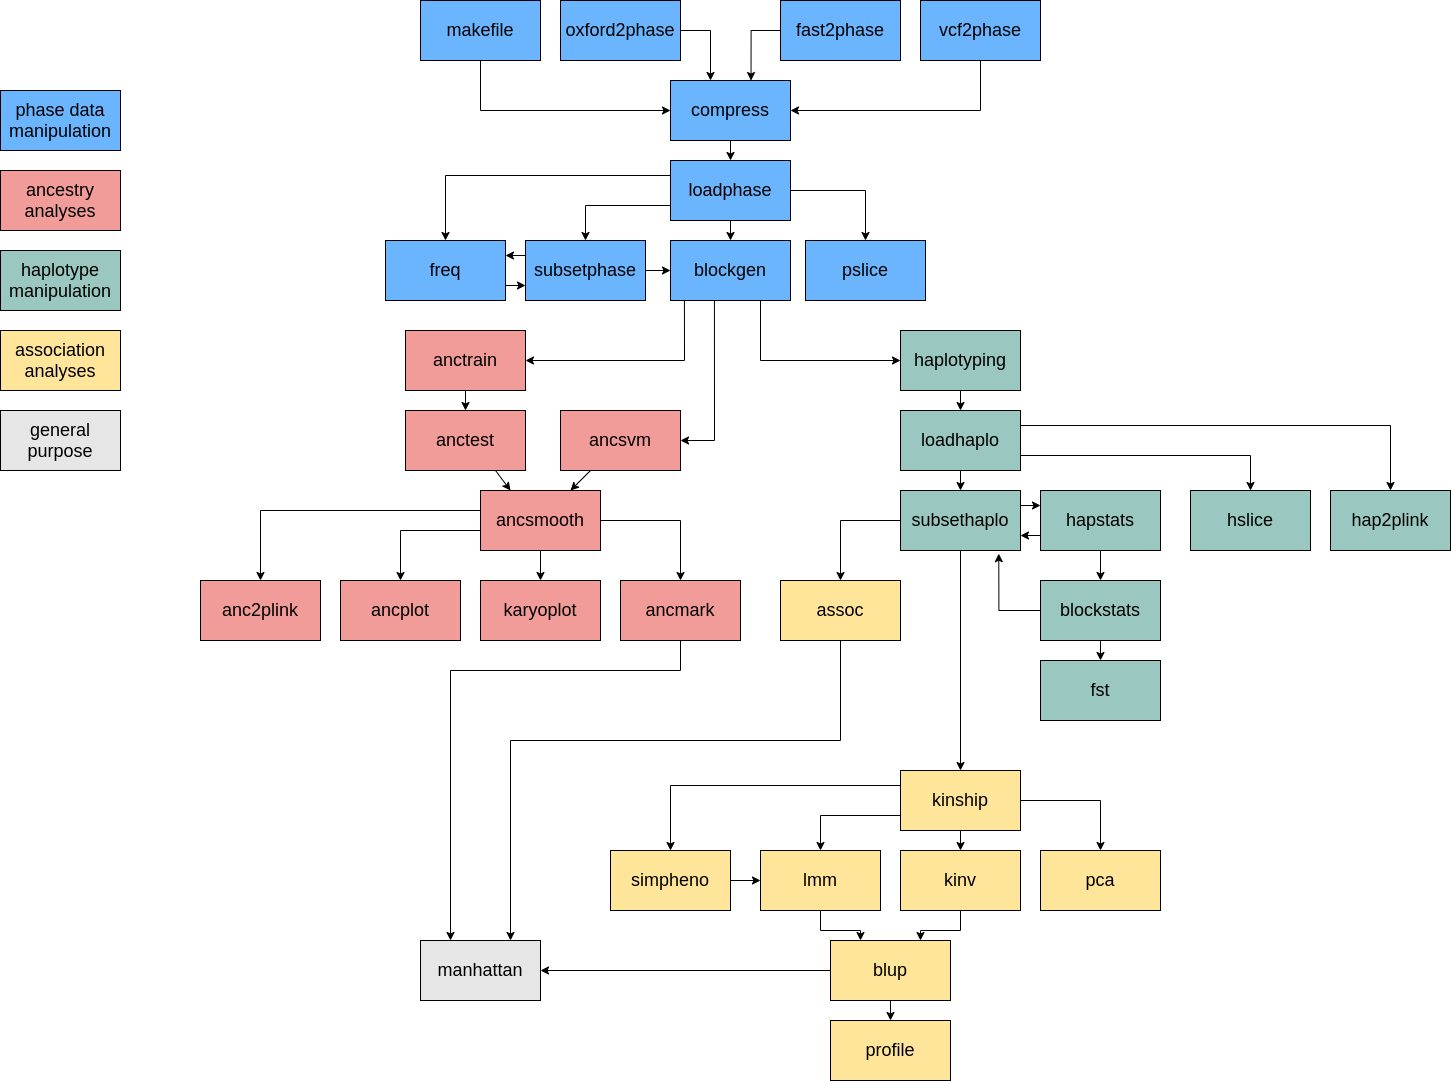
\includegraphics[width=1\linewidth]{diagram_20200718} \caption{Diagram of functions within the package}\label{fig:pressure}
\end{figure}

\pagebreak

\#\#References

N. Amin et al.~A Genomic Background Based Method for Association
Analysis in Related Individuals. PLoS ONE. 2007. 2:e1274.

D. Bates et al.~Fitting Linear Mixed-Effects Models Using lme4. J. Stat.
Soft., 67:1-48.

S. Bolormaa et al.~Detection of chromosome segments of zebu and taurine
origin and their effect on beef production and growth. J. Anim. Sci.
2011. 89:2050-2060.

C. C. Chang et al.~Second-generation PLINK: rising to the challenge of
larger and richer datasets. Gigascience. 2015. 4, 7.

Y. Da. Multi-allelic haplotype model based on genetic partition for
genomic prediction and variance component estimation using SNP markers.
BMC Genet. 2015. 16:144.

B. Devlin and K. Roeder. Genomic control for association studies.
Biometrics. 1999. 55:997-1004.

C. C. Ekine et al.~Why breeding values estimated using familial data
should not be used for genome-wide association studies. G3. 2014.
4:341-347.

R. J. Haasl et al.~Genetic ancestry inference using support vector
machines, and the active emergence of a unique American population. Eur
J Hum Genet. 2013. 21(5):554-62.

J. Listgarten et al.~Improved linear mixed models for genome-wide
association studies. Nat. Methods. 2012. 9:525-526.

R-R. Loh P-R et al.~Reference-based phasing using the Haplotype
Reference Consortium panel. Nat Genet. 2016. 48(11):1443-1448.

D. Meyer et al.~e1071: Misc Functions of the Department of Statistics,
Probability Theory Group (e1071). TU Wien. 2019 R Package Version
1.7-0.1. \url{http://cran.r-project.org/web/packages/e1071/index.html}.

M. Nei. Analysis of Gene Diversity in Subdivided Populations. PNAS.
1973. 70, 3321-3323.

G. N. Norén et al.~Shrinkage observed-to-expected ratios for robust and
transparent large-scale pattern discovery. Stat Methods Med Res. 2013.
22,57-69.

J. O'Connell et al.~A general approach for haplotype phasing across the
full spectrum of relatedness. PLOS Genetics. PLOS Genet. 2014.
10:e1004234.

S. Purcell et al.~PLINK: a tool set for whole-genome association and
population-based linkage analyses. Am. J. Hum. Genet. 2007. 81, 559-575.

I. Strandén and D.J. Garrick. Technical note: derivation of equivalent
computing algorithms for genomic predictions and reliabilities of animal
merit. J Dairy Sci. 2009. 92:2971-2975.

G. R. Svishcheva et al.~Rapid variance components-based method for
whole-genome association analysis. Nat Genet. 2012. 44:1166-1170.

The International HapMap 3 Consortium. Integrating common and rare
genetic variation in diverse human populations. Nature. 2010. 467,
52-58.

P. M. VanRaden. Efficient methods to compute genomic predictions. J.
Dairy. Sci. 2008. 91:4414-4423.

W. M. Venables and B. D. Ripley. Modern Applied Statistics with S.
Fourth Edition. 2002. Springer, New York. ISBN 0-387-95457-0.

H. Wang et al.~Genome-wide association mapping including phenotypes from
relatives without genotypes. Genet Res. 2012. 94:73-83.

J. Yang et al.~Advantages and pitfalls in the application of mixed-model
association methods. Nat. Genet. 2014. 46: 100-106.

\end{document}
